    \documentclass[twoside,11pt]{article}
% HEIN QUOI
% Any additional packages needed should be included after jmlr2e.
% Note that jmlr2e.sty includes epsfig, amssymb, natbib and graphicx,
% and defines many common macros, such as 'proof' and 'example'.
%
% It also sets the bibliographystyle to plainnat; for more information on
% natbib citation styles, see the natbib documentation, a copy of which
% is archived at http://www.jmlr.org/format/natbib.pdf

\usepackage{jmlr2e}
\usepackage{mathtools}
\usepackage{amssymb}
\usepackage{bm}
\usepackage{preamble}
\usepackage{booktabs}
\usepackage{ulem}
\usepackage[most]{tcolorbox}  % Required for the colored box

\newcommand{\Var}{\operatorname{Var}}

% todo
 \setlength {\marginparwidth }{2cm} % TODO: REMOVE THAT later
\usepackage{todonotes}
\definecolor{lightred}{RGB}{120,60,60}
\definecolor{darkred}{RGB}{255,0,0}
\newcommand{\proofread}[1]{{\color{lightred}#1}}
\newcommand{\rewrite}[2]{{\color{darkred}#1}}

\definecolor{gbcolor}{RGB}{220, 160, 180}
\newcommand{\gb}[2][]{\todo[color=gbcolor, caption={GB}, #1]{#2}}
\definecolor{jbcolor}{RGB}{180, 220, 200}
\newcommand{\jb}[2][]{\todo[color=jbcolor, caption={JB}, #1]{#2}}
\definecolor{bpcolor}{RGB}{255, 128, 10}
\newcommand{\bp}[2][]{\todo[color=bpcolor, caption={BP}, #1]{#2}}

% Definitions of handy macros can go here

\newcommand{\dataset}{{\cal D}}
\newcommand{\fracpartial}[2]{\frac{\partial #1}{\partial  #2}}

% Heading arguments are {volume}{year}{pages}{submitted}{published}{author-full-names}

\jmlrheading{1}{2000}{1-48}{4/00}{10/00}{Blanc}

% Short headings should be running head and authors last names

\ShortHeadings{Zq Estimation for Latent Variable Models}{}
\firstpageno{1}

\begin{document}

\title{Z-Estimation for Large-Scale Latent Variable Models}

\author{\name Guillaume Blanc \email guillaume.e.blanc@gmail.com
  \AND
  \name Julien Bodelet \email julien.bodelet@gmail.com
}

\editor{} % lol

\maketitle

\begin{abstract}

Fitting a latent variable model appears to force a choice. Likelihood-based methods---maximum likelihood, EM, variational approximation---are consistent and principled but do not scale: they degrade in the response dimension, in the latent dimension, and under structured priors. Amortized and approximate alternatives scale but surrender statistical guarantees, paying a posterior-misspecification or amortization bias that does not vanish. We show this choice is unnecessary: a designed Z-estimating equation yields a consistent, calibrated estimator for the generative (decoder) parameters that scales to regimes where likelihood-based and variational methods cannot run.

The estimator treats the inference mechanism (the encoder) as given. It forms an estimating function from expectations under a surrogate and subtracts its model expectation, so the induced population moment vanishes at the true decoder \emph{by construction}---for any sufficiently smooth, identifying encoder, not only the exact posterior. We establish consistency and asymptotic normality under a local Jacobian-nonsingularity condition, relate the Jacobian to a perturbation of the Fisher information, and verify it for the Gaussian-proxy generalized linear latent variable model (GLLVM). Surrogate quality affects efficiency and conditioning, never the population root; this decoupling---estimating the decoder without a trained or posterior-exact encoder---is what removes the cost barrier.

Because the centered equations need only samples or expectations under the surrogate---never the marginal likelihood, never a differentiable encoder---they deliver: (i) decoder estimation invariant to the response dimension and immune to amortization bias, with recovery that \emph{improves} as the dimension grows; (ii) calibrated uncertainty, validated to near-nominal coverage by a re-solving parametric bootstrap, in a regime where deterministic observed-information standard errors---including those of standard software---are unreliable; (iii) a bounded-influence, outlier-robust estimator obtained simply by bounding the statistic, with the centering supplying Fisher consistency automatically; and (iv) a Gaussian-process latent variable model (GP-GLLVM) fit at a cost independent of the number of observations, recovering per-factor temporal or spatial length-scales at a scale where likelihood-based and variational methods do not apply. We demonstrate the last on 10x Visium spatial transcriptomics, recovering a scale-resolved, count-native factor decomposition of mouse-brain tissue. These are instances of a single composable construction---the encoder, the statistic, and the latent prior are each free choices---bringing a broader class of scalable, structured latent variable models within reach.

\end{abstract}



\newpage

\listoftodos
\newpage

\section{Notations}
These are our conventions to make the exposition unambiguous. Maybe we will simplify them later. 
\begin{itemize}
    \item A random variable $\Y$ with density $f_{\Y;\,\bt}(\cdot)$ is written $\Y \sim f_{\Y;\,\bt}(\cdot)$, where $\bt$ is the parameter.
    \item Its expectation is written 
    \[
      \mathbb{E}_{f_{\Y;\,\bt}(\cdot)}[\Y] 
      \;=\; \int \y \, f_{\Y;\,\bt}(\y)\, d\y.
    \]
    \item A conditional random variable is written 
    \[
      \Y \mid \Z=\z \;\sim\; f_{\Y \mid \Z;\,\bt}(\cdot \mid \z), 
    \]
    with density $f_{\Y \mid \Z;\,\bt}(\cdot \mid \z)$ and corresponding expectation
    \[
      \mathbb{E}_{f_{\Y \mid \Z;\,\bt}(\cdot \mid \z)}[\Y] 
      \;=\; \int \y \, f_{\Y \mid \Z;\,\bt}(\y \mid \z)\, d\y.
    \]
    \item Joint random variables are whitened as 
    \[
        \Y, \Z \;\sim\; f_{\Y,\Z;\,\bt}(\cdot, \cdot)
    \]
    
    \item \textbf{Remark 1}: We use $\cdot$ as argument when we do not refer to a specific pre-image. We write for instance $f_{\Z}(\cdot)$ instead of $f_{\Z}(\z)$ to specify the whole density, not simply evaluated at a particular $\z$. When we want to evaluate it at a particular $\z$, we use the latter.
    \item \textbf{Remark 2}: We prefer to write using Expectations instead of integrals because expectations carry intuition and is easier to read and manipulate.
\end{itemize}
\newpage


\newpage

\section{Introduction}

Latent variable models are a standard way to represent complex dependence in multivariate data by introducing an unobserved variable $\Z$ that explains structure in an observed variable $\Y$.
They underpin classical random-effects models, generalized latent variable models, and modern deep generative models.
A typical specification is
\begin{align}
\Z &\sim f_{\Z}, \nonumber\\
\Y \mid \Z &\sim f_{\Y\mid \Z;\,\bt},
\label{eq:intro_generative}
\end{align}
where $\bt\in\bm\Theta$ denotes the decoder (generative) parameters.
Inference for $\bt$ is typically based on the marginal likelihood of $\Y$,
which requires integrating out $\Z$, and is often implemented through posterior expectations under $f_{\Z\mid\Y;\bt}$.
Outside of a few special cases, these quantities are not available in closed form, and practical methods therefore replace $f_{\Z\mid\Y;\bt}$ by a tractable surrogate $q_{\Z\mid\Y;\bt}$.

This includes variational EM and modern amortized inference methods such as variational autoencoders (VAEs), where a surrogate posterior mechanism $q_{\Z\mid\Y;\bt}$ is induced by an encoder network shared across observations \citep{dempster1977maximum,jordan1999introduction,kingma2014autoencoding,blei2017variational}.
While these approaches scale well, they can induce systematic bias when the surrogate posterior mechanism $q_{\Z\mid\Y;\bt}$ is misspecified, underspecified, or reused under distribution shift.
In particular, with amortized inference, mismatch between the encoder family and the true posterior---together with the additional gap introduced by amortization---can propagate into biased decoder updates that persist even as the sample size grows (often referred to as amortization bias or the amortization gap; see, e.g., \citealp{cremer2018inference}).
Several lines of work aim to reduce the impact of mismatch between $q_{\Z\mid\Y}$ and $f_{\Z\mid\Y;\bt}$ by improving the variational approximation itself, including stochastic and black-box variational inference \citep{hoffman2013svi,ranganath2014bbvi}, richer variational families such as normalizing flows \citep{rezende2015flows}, tighter bounds such as importance-weighted objectives \citep{burda2016iwae}, and hybrid approaches that refine amortized solutions with per-instance optimization \citep{kim2018semiamortized}.

This paper asks a simple question:
\emph{can we estimate the decoder parameters $\bt$ consistently despite using an approximate, misspecified, or reused surrogate posterior mechanism $q_{\Z\mid\Y;\bt}$?}
Our answer is yes, under a local identification condition. The key idea is to replace the usual surrogate-based decoder update by a \emph{centered estimating equation}: we form an estimating function $\psi_q(\bt;\Y)$ from expectations under the surrogate and subtract its model expectation under $f_{\Y;\bt}$. This guarantees that the induced population moment vanishes at the true decoder by construction, regardless of whether the surrogate posterior is correct. The surrogate may therefore be a learned encoder, a pretrained module, a MAP approximation, or even a point imputer $q_{\Z\mid\Y}(\cdot\mid y)=\delta_{\tilde z(y)}(\cdot)$. In all such cases, centering corrects the population target, so posterior quality affects efficiency rather than the population root. Our focus is decoder estimation conditional on a chosen surrogate inference mechanism. Here ``conditional'' means that the surrogate mechanism is treated as given when defining the estimating equations: the surrogate family may still be indexed by the decoder parameter, but it is not itself jointly re-estimated as a nuisance component in the asymptotic analysis. In particular, the most immediate use cases are settings where a surrogate is already available---for example through pretraining, amortized inference, encoder reuse under shift, or deterministic imputation---and the goal is to estimate or refine decoder parameters without relying on posterior correctness.

\paragraph{Contributions.}
We make four main contributions.
First, we introduce the $Z_q$ estimator, a centered Z-estimation procedure for decoder parameters that is consistent for \emph{any} surrogate posterior, and establish its consistency and asymptotic normality under a local Jacobian nonsingularity condition (Section~\ref{sec:asymptotics}).
Second, we relate the Jacobian to a perturbation of the Fisher information, giving interpretable sufficient conditions for local identification, and we \emph{verify} them for the Gaussian-proxy GLLVM (Appendix~\ref{apx:gllvm-identification}).
Third, we show the construction makes two practically important estimators essentially free, because it never needs the marginal likelihood or a differentiable encoder: a \emph{robust} decoder estimator with bounded influence in the response---obtained by bounding the statistic, the centering supplying Fisher consistency automatically---and a \emph{scalable} estimator whose per-step cost is independent of the response and sample sizes through response/observation subsampling.
Fourth, we develop the \emph{GP-GLLVM} (Section~\ref{sec:gpgllvm}): a Gaussian-process latent-variable model estimated likelihood-free at a cost independent of the number of observations, and apply it to spatial transcriptomics---to our knowledge the first count-native Gaussian-process factor analysis at this scale.
We focus throughout on decoder estimation conditional on a given surrogate \emph{mechanism}, not the full joint asymptotics of simultaneous encoder--decoder training.

\paragraph{Empirical evaluation.}
Our experiments (Section~\ref{sec:sims}) target the method's claims where the truth is known.
(i) Under a deliberately misspecified or underspecified encoder, $Z_q$ recovers the decoder where ELBO training is biased, and its accuracy is \emph{invariant to the response dimension} $p$ while a variational autoencoder degrades sharply.
(ii) In the maximum-likelihood estimator's own regime (small dense Poisson GLLVMs), $Z_q$ with an asymptotically-free loading ridge is competitive with a state-of-the-art variational MLE.
(iii) A bounded-influence variant is flat against outlier magnitude and degrades gracefully with the contamination fraction up to its breakdown point.
(iv) The GP-GLLVM fits at a cost independent of $n$---up to millions of observations---recovers per-factor length-scales, and yields an interpretable scale-resolved decomposition of real spatial-transcriptomics data.

\paragraph{On identification.}
Local identification of the $Z_q$ estimator reduces to nonsingularity of the
Jacobian of the induced population moment map.
This condition is model-specific, as in classical likelihood theory for latent-variable models,
and depends on how the decoder parameters enter the conditional distribution.
A full characterization of identification across all latent-variable models
is therefore beyond the scope of this work.
We provide explicit verification in canonical settings (e.g., Gaussian factor models)
and derive general sufficient conditions based on perturbations of the Fisher information.
In addition, we show that among a natural class of centered estimating equations,
the proposed construction minimizes first-order sensitivity to posterior misspecification,
providing a robustness optimality result within that class.


\paragraph{Organization.}
Section~\ref{sec:method} defines the $Z_q$ estimating equations and relates them to classical likelihood identities in latent variable models.
Section~\ref{sec:asymptotics} provides asymptotic theory and identification conditions.
Section~\ref{sec:gpgllvm} develops the scalable GP-GLLVM.
Section~\ref{sec:sims} reports the empirical study.


% ============================== 


\section{Method}
\label{sec:method}

\subsection{Model setup}

We consider a parametric latent variable model in which an observed random vector
$\Y \in \mathcal Y \subseteq \mathbb R^p$ is generated from an unobserved latent variable
$\Z \in \mathcal Z \subseteq \mathbb R^q$ according to
\[
(\Y,\Z) \sim f_{\Y,\Z;\bt}(\cdot,\cdot)
= f_{\Y\mid\Z;\bt}(\cdot\mid\cdot)\,f_\Z(\cdot),
\]
where $f_\Z$ is a known prior distribution and $\bt\in\Theta\subseteq\mathbb R^r$ denotes
the decoder parameters of interest. The latent variable $\Z$ is never observed.

Throughout, we assume that the conditional distribution $f_{\Y\mid\Z;\bt}$ belongs to
a canonical exponential family, so that for $(\y,\z)\in\mathcal Y\times\mathcal Z$,
\[
f_{\Y\mid\Z;\bt}(\y\mid\z)
=
\exp\!\left\{
T(\y)^\top \eta(\z,\bt)
-
A\!\bigl(\eta(\z,\bt)\bigr)
+
B(\y)
\right\},
\]
where $T(\y)$ is a sufficient statistic, $\eta(\z,\bt)$ is the natural parameter, and
$A(\cdot)$ is the log-partition function. This formulation covers generalized linear
latent variable models and decoder networks with exponential-family output layers.

Because $\Z$ is unobserved, inference for $\bt$ is typically based on the marginal likelihood
\[
f_{\Y;\bt}(\y)=\int f_{\Y\mid\Z;\bt}(\y\mid\z)\,f_\Z(\z)\,d\z.
\]
Under standard regularity conditions, the maximum likelihood estimator (MLE) is a root of
the empirical score. Writing
\[
s(\bt;\y)\vcentcolon=\nabla_\bt \log f_{\Y;\bt}(\y),
\]
the MLE $\hat\bt_{\mathrm{MLE}}$ satisfies
\begin{equation}
\frac{1}{n}\sum_{i=1}^n s(\bt;\y_i)=0.
\label{eq:mle_score_eq}
\end{equation}

In latent variable models, the marginal score admits the posterior-expectation representation
\begin{equation}
s(\bt;\y)
=
\mathbb{E}_{f_{\Z\mid\Y;\bt}(\cdot\mid \y)}
\!\left[
\nabla_\bt \log f_{\Y,\Z;\bt}(\y,\Z)
\right],
\label{eq:score_posterior_form}
\end{equation}
which follows from standard identities (see Appendix~\ref{apx:mle-estimating-equations}) and
coincides with the quantity used in the E-step of the EM algorithm.

\subsection{Score decomposition and the matching form of the MLE}

In the exponential-family setting above, the posterior form \eqref{eq:score_posterior_form}
can be written as
\begin{equation}
s(\bt;\y)
=
\mathbb{E}_{f_{\Z\mid\Y;\bt}(\cdot\mid \y)}
\!\left[
D(\Z;\bt)^\top\bigl(T(\y)-\mu(\Z;\bt)\bigr)
\right],
\label{eq:score_expfam}
\end{equation}
where $D(\z;\bt)=\partial\eta(\z,\bt)/\partial\bt$ and
$\mu(\z;\bt)=\E_{f_{\Y\mid\Z;\bt}(\cdot\mid \z)}[T(\Y)]$.
Expanding \eqref{eq:score_expfam} yields
\begin{equation}
s(\bt;\y)
=
\mathbb{E}_{f_{\Z\mid\Y;\bt}(\cdot\mid \y)}\!\big[D(\Z;\bt)^\top T(\y)\big]
-
\mathbb{E}_{f_{\Z\mid\Y;\bt}(\cdot\mid \y)}\!\big[D(\Z;\bt)^\top \mu(\Z;\bt)\big].
\label{eq:score_two_terms}
\end{equation}

Given i.i.d.\ observations $\y_1,\dots,\y_n \sim f_{\Y;\bt_0}$, plugging \eqref{eq:score_two_terms}
into \eqref{eq:mle_score_eq} shows that the MLE satisfies a matching of two empirical averages:
\begin{equation}
\frac{1}{n}\sum_{i=1}^n
\mathbb{E}_{f_{\Z\mid\Y;\bt}(\cdot\mid \y_i)}\!\big[D(\Z;\bt)^\top T(\y_i)\big]
\;=\;
\frac{1}{n}\sum_{i=1}^n
\mathbb{E}_{f_{\Z\mid\Y;\bt}(\cdot\mid \y_i)}\!\big[D(\Z;\bt)^\top \mu(\Z;\bt)\big].
\label{eq:mle_matching}
\end{equation}

The left-hand side is anchored by the observed statistic $T(\y_i)$. By contrast, the
right-hand side replaces $T(\y_i)$ by the model-implied conditional mean
$\mu(\Z;\bt)$ and depends on the data only through the posterior
$f_{\Z\mid\Y;\bt}$. This second term is therefore the fragile part of the score equation:
when the generally intractable posterior is replaced by a surrogate
$q_{\Z\mid\Y}$, the induced target is typically no longer calibrated, and the resulting
plug-in equations are generally inconsistent.

Much of the existing literature addresses this problem by improving the approximation
$q_{\Z\mid\Y}$ so that it more closely matches $f_{\Z\mid\Y;\bt}$. Our approach is
different. Rather than trying to repair the surrogate posterior itself, we replace the
target in \eqref{eq:mle_matching} by a model-based centering term that restores the
correct population moment condition even when the surrogate is misspecified.

\subsection{The $Z_q$ estimator}
\label{sec:zq_estimator}

Our construction keeps the data-anchored term from \eqref{eq:mle_matching}, with
$q_{\Z\mid\Y}$ substituting for the intractable posterior, and centers it under the
marginal model. Define
\begin{equation}
\psi(\bt;\y)
:=
\mathbb{E}_{q_{\Z\mid\Y;\bt}(\cdot\mid \y)}\!\big[D(\Z;\bt)^\top T(\y)\big].
\label{eq:psi_theta_dep_method}
\end{equation}
We then consider the centered estimating map
\begin{equation}
\Psi_n(\bt)
:=
\frac{1}{n}\sum_{i=1}^n \psi(\bt;\y_i)
-
\mathbb{E}_{f_{\Y;\bt}}\!\left[\psi(\bt;\Y)\right].
\label{eq:Psi_n_general}
\end{equation}
Its population counterpart is
\[
\Psi(\bt)
:=
\mathbb E_{f_{\Y;\bt_0}}\!\left[\psi(\bt;\Y)\right]
-
\mathbb E_{f_{\Y;\bt}}\!\left[\psi(\bt;\Y)\right],
\]
so that
\[
\Psi(\bt_0)=0.
\]

This centering step is the key idea. It replaces the misspecification-sensitive target in
\eqref{eq:mle_matching} by a model expectation that exactly matches the empirical term at
the truth in population. As a result, the population moment condition is correct by
construction, regardless of whether $q_{\Z\mid\Y}$ coincides with the true posterior.

A crucial design choice is the form of $\psi_q$. One might try to center a more direct
approximation of the marginal score, but such constructions need not yield locally
identifying equations under posterior misspecification. By centering the data-anchored
term from the exponential-family decomposition \eqref{eq:score_two_terms}, we retain the
part of the score equation that is directly tied to the observed statistic $T(\y)$ while
moving the misspecification-sensitive component into the model-based centering term. This
choice leads to estimating equations that remain locally identifying under mild conditions,
developed in Section~\ref{sec:asymptotics}.

We therefore define the estimator as follows.

\begin{definition}[$Z_q$ estimator]
\label{def:Zq}
The $Z_q$ estimator $\hat\bt_n$ is any solution of $\Psi_n(\bt)=0$.
\end{definition}

The practical consequence is simple: decoder estimation requires only expectations or samples
under the surrogate $q_{\Z\mid\Y}$. It does not require differentiating through the mechanism
used to produce that surrogate. The same estimating equations therefore apply to learned
encoders, pretrained modules, MAP-based approximations, and degenerate point-imputation rules
$q_{\Z\mid\Y;\bt}(\cdot\mid \y)=\delta_{\tilde z(\y)}(\cdot)$. This is particularly useful in
regimes where a surrogate inference mechanism is already available and decoder parameters must
be estimated or refined despite misspecification, reuse, or distribution shift. The role of the
surrogate is to define the estimating function; centering then restores the correct population target.

In practice, the surrogate may be obtained in many ways and may itself depend on the
current decoder, for example through amortized inference or a MAP rule. This does not
conflict with our use of the word ``fixed'': what is treated as given is the surrogate
\emph{mechanism}, that is, the rule $\bt \mapsto q_{\Z\mid\Y;\bt}$ entering the estimating
equation. The surrogate need not be pointwise independent of $\bt$; rather, it is not
jointly re-estimated as an additional nuisance object within the asymptotic analysis.
Those broader $\bt$-indexed surrogate mechanisms are handled in
Section~\ref{sec:asymptotics}. For the present section, the estimator is completely defined
by \eqref{eq:Psi_n_general}: any procedure that supplies the required expectations or samples
under a chosen surrogate can be inserted into the same centered estimating equations.


\paragraph{Alternating refinement.}
In practice, one may alternate between updating the surrogate posterior and updating the decoder. Starting from a current decoder value $\bt^{(t)}$, one may train a surrogate $q^{(t)}_{\Z\mid\Y}$---for instance on synthetic data generated under $\bt^{(t)}$ or by a standard variational objective---then freeze this surrogate and compute a decoder update by solving the centered estimating equations with $q^{(t)}_{\Z\mid\Y}$ held fixed. Repeating this procedure can improve empirical performance, but the resulting alternating scheme is an optimization heuristic rather than a single Z-estimator. Our asymptotic theory applies to each decoder update conditional on the current frozen surrogate, and in particular to the final stage once the encoder has been fixed. Thus the present analysis covers decoder refinement with a learned or reused surrogate mechanism, but not the full joint asymptotic behavior of simultaneous encoder--decoder training in which encoder parameters are themselves estimated from the same sample throughout the coupled procedure.



% ==============================================================


\section{Asymptotic Theory}
\label{sec:asymptotics}

This section places the proposed estimator in the classical Z-estimation framework
and isolates the main model-specific issue: local identification. We write the
surrogate posterior as $q_{\Z\mid\Y;\bt}$ to allow for amortized encoders,
MAP-based rules, pretrained black-box modules, and other $\bt$-indexed
approximation mechanisms, viewed as part of the estimating map. The surrogate need
not equal the true posterior $f_{\Z\mid\Y;\bt}$ and may remain misspecified. The
analysis does not treat separate encoder parameters as jointly estimated nuisance
quantities. Rather, it studies decoder estimation conditional on a given surrogate
\emph{mechanism}: the rule $\bt \mapsto q_{\Z\mid\Y;\bt}$ is taken as part of the
estimating equation, even though the resulting surrogate may still depend on $\bt$.

The main structural result is that, after centering, derivatives of the surrogate
mechanism do not contribute to the first-order Jacobian at the truth. As a result,
posterior misspecification changes local conditioning and efficiency, but not the
population root.

\subsection{Population estimating equations}

Define
\begin{equation}
\psi(\bt;\y)
:=
\mathbb E_{q_{\Z\mid\Y;\bt}(\cdot\mid \y)}
\!\left[D(\Z;\bt)^\top T(\y)\right],
\label{eq:psi_theta_dep}
\end{equation}
and recall the sample estimating map
\[
\Psi_n(\bt)
=
\frac{1}{n}\sum_{i=1}^n \psi(\bt;\y_i)
-
\mathbb E_{f_{\Y;\bt}}\!\left[\psi(\bt;\Y)\right].
\]
Its population counterpart is
\[
\Psi(\bt)
=
\mathbb E_{f_{\Y;\bt_0}}\!\left[\psi(\bt;\Y)\right]
-
\mathbb E_{f_{\Y;\bt}}\!\left[\psi(\bt;\Y)\right].
\]
By construction,
\[
\Psi(\bt_0)=0.
\]
This identity holds for any surrogate family $q_{\Z\mid\Y;\bt}$, whether
well specified or misspecified. Misspecification therefore does not alter the
population root; it enters only through the local geometry of $\Psi$ around
$\bt_0$.

\subsection{Jacobian identity and cancellation of chain-rule terms}

Let $s(\bt;\Y)=\nabla_\bt \log f_{\Y;\bt}(\Y)$ denote the marginal score. Under
standard regularity conditions allowing differentiation under the integral sign,
the score identity implies that for any sufficiently smooth $g(\bt,\Y)$,
\[
\nabla_\bt \mathbb E_{f_{\Y;\bt}}\!\left[g(\bt,\Y)\right]
=
\mathbb E_{f_{\Y;\bt}}\!\left[\nabla_\bt g(\bt,\Y)\right]
+
\mathbb E_{f_{\Y;\bt}}\!\left[g(\bt,\Y)s(\bt;\Y)^\top\right].
\]
Applying this identity with $g(\bt,\Y)=\psi(\bt;\Y)$ yields
\begin{align}
\nabla_\bt \Psi(\bt)
&=
\mathbb E_{f_{\Y;\bt_0}}\!\left[\nabla_\bt \psi(\bt;\Y)\right]
-
\nabla_\bt \mathbb E_{f_{\Y;\bt}}\!\left[\psi(\bt;\Y)\right]
\nonumber\\
&=
\mathbb E_{f_{\Y;\bt_0}}\!\left[\nabla_\bt \psi(\bt;\Y)\right]
-
\mathbb E_{f_{\Y;\bt}}\!\left[\nabla_\bt \psi(\bt;\Y)\right]
-
\mathbb E_{f_{\Y;\bt}}\!\left[\psi(\bt;\Y)s(\bt;\Y)^\top\right].
\label{eq:jacobian_pre_cancel}
\end{align}
Evaluating at $\bt=\bt_0$, the two derivative terms cancel exactly:
\begin{equation}
\nabla_\bt \Psi(\bt_0)
=
-
\mathbb E_{f_{\Y;\bt_0}}\!\left[\psi(\bt_0;\Y)s(\bt_0;\Y)^\top\right].
\label{eq:jacobian_cancel}
\end{equation}
Equivalently, the Jacobian at the truth is
\begin{equation}
A(\bt_0)
:=
-\nabla_\bt \Psi(\bt_0)
=
\mathbb E_{f_{\Y;\bt_0}}\!\left[\psi(\bt_0;\Y)s(\bt_0;\Y)^\top\right].
\label{eq:jacobian_final}
\end{equation}

Equation~\eqref{eq:jacobian_cancel} is the main structural identity of the
theory. The object $\nabla_\bt \psi(\bt;\Y)$ contains all direct and indirect
dependence of the estimating function on $\bt$, including any chain-rule terms
arising through the surrogate posterior $q_{\Z\mid\Y;\bt}$. Yet these terms
disappear from the Jacobian of the centered population equation. Thus the first-order asymptotic analysis depends on the surrogate only through
the value of $\psi(\bt_0;\Y)$, not through derivatives of the encoder or of the
learning procedure used to obtain it. In this sense, the surrogate mechanism is
treated as given, even when the surrogate family itself is indexed by $\bt$.

\subsection{Consistency and asymptotic normality}

We now impose standard assumptions for Z-estimation.

\begin{assumption}[Uniform convergence]
\label{ass:uniform-conv}
With probability one,
\[
\sup_{\bt\in\Theta}
\bigl\|
\Psi_n(\bt)-\Psi(\bt)
\bigr\|
\longrightarrow 0
\qquad\text{as } n\to\infty.
\]
\end{assumption}

\begin{assumption}[Local nonsingularity]
\label{ass:nonsingularity}
The map $\Psi$ is continuously differentiable in a neighborhood of $\bt_0$, and
the Jacobian matrix $A(\bt_0)$ in \eqref{eq:jacobian_final} is nonsingular.
\end{assumption}

Assumption~\ref{ass:uniform-conv} is standard. Assumption~\ref{ass:nonsingularity}
is the local identification condition. The centered construction guarantees that
$\bt_0$ is always a population root; the substantive question is whether the
moment map remains locally informative around that root.

\begin{theorem}[Consistency and asymptotic normality]
\label{thm:Zq-main}
Suppose Assumptions~\ref{ass:uniform-conv} and~\ref{ass:nonsingularity} hold.
Then there exists a sequence of solutions $\hat\bt_n$ to $\Psi_n(\bt)=0$ such that
\[
\hat\bt_n \xrightarrow{p} \bt_0.
\]
Moreover,
\[
\sqrt{n}\,(\hat\bt_n-\bt_0)
\Longrightarrow
\mathcal N\!\bigl(0,\Sigma\bigr),
\]
with sandwich covariance
\[
\Sigma
=
A(\bt_0)^{-1}
B(\bt_0)
A(\bt_0)^{-\top},
\qquad
B(\bt_0)
=
\Var_{f_{\Y;\bt_0}}\!\bigl(\varphi(\bt_0;\Y)\bigr),
\]
where
\[
\varphi(\bt;\Y)
=
\psi(\bt;\Y)-\mathbb E_{f_{\Y;\bt}}\!\left[\psi(\bt;\Y)\right].
\]
\end{theorem}

Theorem~\ref{thm:Zq-main} is a direct application of standard Z-estimation
theory \citep[Theorems 5.9 and 5.41]{vandervaart1998}. The centering term in
$\Psi_n$ contributes to the influence function through the centered variable
$\varphi(\bt_0;\Y)$, which has mean zero under $f_{\Y;\bt_0}$. Its interpretation
is central here: posterior misspecification does not alter the population root,
and even when the surrogate depends on $\bt$, its derivative does not enter the
first-order Jacobian thanks to \eqref{eq:jacobian_cancel}.

\subsection{Identification via a Fisher-information perturbation}

The Jacobian in \eqref{eq:jacobian_final} can be compared directly to the Fisher
information. Add and subtract the marginal score to obtain
\begin{align}
A(\bt_0)
&=
\mathbb E\!\left[s(\bt_0;\Y)s(\bt_0;\Y)^\top\right]
+
\mathbb E\!\left[(\psi(\bt_0;\Y)-s(\bt_0;\Y))\,s(\bt_0;\Y)^\top\right]
\nonumber\\
&=
\mathcal I(\bt_0)+M(\bt_0),
\label{eq:fisher_perturb}
\end{align}
where
\[
\mathcal I(\bt_0)
=
\mathbb E\!\left[s(\bt_0;\Y)s(\bt_0;\Y)^\top\right]
\]
is the Fisher information and
\[
M(\bt_0)
:=
\mathbb E\!\left[(\psi(\bt_0;\Y)-s(\bt_0;\Y))\,s(\bt_0;\Y)^\top\right]
\]
measures the discrepancy between the centered estimating function and the true
score.

Equation~\eqref{eq:fisher_perturb} shows that the Jacobian of the $Z_q$
equations is a perturbation of the Fisher information. This gives a transparent
interpretation of the method: centering fixes the population root, while the
surrogate affects local identification only through how far the induced moment
function deviates from the score at the truth.

The following condition provides a convenient sufficient criterion.

\begin{assumption}[Controlled deviation from the score]
\label{ass:jacobian-perturbation}
The Fisher information $\mathcal I(\bt_0)$ is nonsingular, and
\[
\bigl\|
\mathcal I(\bt_0)^{-1/2}
\,M(\bt_0)\,
\mathcal I(\bt_0)^{-1/2}
\bigr\|_{\mathrm{op}}
<1.
\]
\end{assumption}

\begin{proposition}[A sufficient condition for local identification]
\label{prop:jacobian-neumann}
Under Assumption~\ref{ass:jacobian-perturbation}, the Jacobian $A(\bt_0)$ is
nonsingular.
\end{proposition}

\begin{proof}
Let
\[
\widetilde M
=
\mathcal I(\bt_0)^{-1/2}
M(\bt_0)
\mathcal I(\bt_0)^{-1/2}.
\]
Then \eqref{eq:fisher_perturb} may be rewritten as
\[
A(\bt_0)
=
\mathcal I(\bt_0)^{1/2}
\bigl(I+\widetilde M\bigr)
\mathcal I(\bt_0)^{1/2}.
\]
If $\|\widetilde M\|_{\mathrm{op}}<1$, then $I+\widetilde M$ is invertible by
the Neumann series, hence so is $A(\bt_0)$.
\end{proof}

Proposition~\ref{prop:jacobian-neumann} makes explicit the robustness of the
construction. Surrogate quality affects local conditioning and asymptotic
variance, but not the correctness of the population root.

\subsection{Efficiency}

The asymptotic variance of the $Z_q$ estimator is
\[
\Sigma
=
A(\bt_0)^{-1}
B(\bt_0)
A(\bt_0)^{-\top},
\qquad
B(\bt_0)
=
\Var\!\bigl(\varphi(\bt_0;\Y)\bigr),
\]
where
\[
\varphi(\bt_0;\Y)
=
\psi(\bt_0;\Y)-\mathbb E\!\left[\psi(\bt_0;\Y)\right].
\]
Thus efficiency depends on the surrogate posterior through both the Jacobian
and the variability of the centered estimating function. More accurate
surrogates may improve conditioning and reduce variance, but there is no
general reason for the oracle choice
$q_{\Z\mid\Y;\bt_0}=f_{\Z\mid\Y;\bt_0}$ to recover the MLE or attain Fisher
efficiency, since the centered estimating function is not, in general, the
marginal score.

The relevant conclusion is therefore weaker and more appropriate here:
posterior quality affects \emph{efficiency}, but consistency follows from
centering together with local identification.

\paragraph{Overidentification and connection to GMM.}
The present construction uses a single sufficient statistic $T(y)$ in the estimating equation, yielding a just-identified system with one moment per parameter.
It is straightforward to stack $K$ statistics $T_1,\ldots,T_K$ and form an overidentified system of $Kd$ moment conditions for $d$ parameters.
Each individual system $\Psi_n^{(k)}(\bt)=0$ is consistent by the same centering argument, and their combination fits naturally within the generalized method of moments (GMM) framework of \citet{hansen1982large}.
The optimal GMM weight matrix then trades off the $K$ moment conditions to minimize asymptotic variance, potentially improving efficiency over any single $T_k$.
In practice, a simple equal-weight average $T(y) = K^{-1}\sum_k T_k(y)$ already combines the conditions and remains just-identified, though without the variance reduction of optimal weighting.
We do not pursue this extension here, but note that the $Z_q$ framework is a natural vehicle for it.

\paragraph{Gaussian factor analysis as a benchmark case.}
The efficiency discussion above should not be read as saying that centered estimation with a surrogate posterior is necessarily inefficient relative to likelihood-based methods. In some classical latent-variable models, the centered equations recover the efficient score exactly even when the surrogate itself is extremely crude. In particular, in Gaussian factor analysis, if \(q_{\Z\mid\Y}\) is taken to be a point mass at the posterior mode, then the resulting \(Z_q\) estimating equations coincide with the marginal score equations. Thus the \(Z_q\) estimator equals the maximum likelihood estimator and is Fisher efficient in this case. This happens because, in the linear-Gaussian setting, the posterior mean equals the MAP and the complete-data score has a structure for which replacing the posterior by its mean/MAP leaves the centered estimating equation \eqref{eq:Psi_n_general} unchanged; see Appendix~\ref{apx:fa-efficiency}.



\subsection{The large-\texorpdfstring{$p$}{p}, small-\texorpdfstring{$n$}{n} regime}
\label{sec:large-p}

A practically important regime that is not captured by standard asymptotic analysis in $n$ is the one in which the observation dimension $p$ is large relative to the sample size $n$, as is typical in single-cell RNA sequencing ($p \sim 10^4$ genes, $n \sim 10^3$--$10^4$ cells).
In this setting the $Z_q$ estimator with a parameter-free Gaussian proxy encoder has a qualitatively different behaviour from a VAE encoder.

\paragraph{The proxy encoder concentrates in $p$.}
The Gaussian proxy posterior sets $\mu(y;\theta) = \Sigma_z W_z^\top T(y)$, a weighted sum over $p$ features. By a law-of-large-numbers argument in $p$, this sum concentrates around its expectation at rate $1/\sqrt{p}$, independently of $n$. Concretely, as $p\to\infty$ with $n$ fixed:
\begin{itemize}
  \item the MAP point $\hat z(y) \to \mathbb{E}[Z \mid Y = y; \theta]$ in the Gaussian GLLVM, so the proxy becomes the true posterior mean;
  \item the posterior becomes increasingly peaked, and the MAP assignment recovers the exact posterior mode;
  \item the $Z_q$ estimating equations therefore converge to the true complete-data score equations, and the estimator behaves like a GLM fit with known latent variables.
\end{itemize}
This is the sense in which the method improves with $p$: the encoder is \emph{self-correcting} through concentration, with no additional data required.

\paragraph{Contrast with amortised VAE encoders.}
A neural network encoder $q_\phi(z\mid y)$ must learn from the $n$ training observations how to map $\mathbb{R}^p \to \mathbb{R}^q$. Its generalisation gap scales with the number of parameters divided by $n$, irrespective of $p$. As $p$ grows the VAE encoder gains no benefit from the additional signal, but the number of input weights grows linearly, increasing the risk of overfitting or slow convergence. The $Z_q$ proxy encoder, having zero learnable parameters, is immune to this problem.

\paragraph{Empirical confirmation.}
Simulations with a sparse Poisson GLLVM ($q=2$, $p \in \{20\}$, $n=1000$, loading scale $\sigma_W = 0.3$) confirm the qualitative picture and add a striking finding: the proxy encoder outperforms the VAE even in the \emph{large-$n$/small-$p$} regime, precisely where amortised inference is expected to be most competitive.
At $p=20$, $n=1000$ --- a setting with 50 observations per input dimension, far above typical deep-learning data requirements --- the Gauss-posterior proxy with $T(y) = (\log(1+y)+\sqrt{y})/2$ achieves Procrustes error $0.101$ versus $0.143$ for a well-tuned VAE (with warm-up, learning-rate annealing, and early stopping), a 30\% improvement.
The result holds across seeds.

This suggests the amortisation gap is a \emph{structural} property of the ELBO objective rather than a data-starvation artefact: even with ample data the joint optimisation of encoder and decoder under the KL-regularised objective creates a landscape in which the encoder does not converge to the true posterior, and the resulting gradient bias in the decoder update persists.
The $Z_q$ proxy sidesteps this entirely; the encoder is never trained, never overfits, and never induces gradient bias in the decoder.

\todo[color=yellow]{TODO: add p-sweep figure showing Procrustes vs.\ $p$ for best ZQE arm and VAE.}

\subsection{Variance estimation and inference}
\label{sec:variance}

The asymptotic normality result of Theorem~\ref{thm:Zq-main} provides a basis for statistical inference on \(\bt_0\). In particular,
\[
\sqrt{n}\,(\hat\bt_n-\bt_0)
\Longrightarrow
\mathcal N\!\bigl(0,\Sigma\bigr),
\qquad
\Sigma
=
A(\bt_0)^{-1}B(\bt_0)A(\bt_0)^{-\top}.
\]
Thus, confidence intervals and Wald-type procedures require a consistent estimator of the asymptotic covariance matrix \(\Sigma\).

A direct plug-in approach is generally inconvenient in latent-variable models. The score \(s(\bt;Y)\) is typically unavailable in closed form, and the Jacobian \(A(\bt_0)\) involves population expectations under the unknown data-generating distribution. Moreover, our goal is precisely to avoid differentiating through the surrogate posterior mechanism. For inference, it is therefore natural to use resampling-based procedures that exploit the centered Z-estimation structure of the problem.

\paragraph{Freezing the surrogate posterior.}
A key observation is that freezing the surrogate posterior at the fitted decoder value does not affect the first-order asymptotic distribution. Let
\[
\widehat q(\cdot\mid y)
:=
q_{\Z\mid\Y;\hat\bt_n}(\cdot\mid y),
\]
and define the frozen estimating map
\[
\Psi_n^{\mathrm{fr}}(\bt)
=
\frac{1}{n}\sum_{i=1}^n \psi_{\widehat q}(\bt;\y_i)
-
\mathbb E_{f_{\Y;\bt}}\!\left[\psi_{\widehat q}(\bt;\Y)\right].
\]
Denote by \(\hat\bt_n^{\mathrm{fr}}\) any solution of
\[
\Psi_n^{\mathrm{fr}}(\bt)=0.
\]
The justification is the same cancellation identity as in \eqref{eq:jacobian_cancel}. In the original estimator, the surrogate may depend on \(\bt\), but its derivative does not contribute to the first-order Jacobian at the truth. Consequently, replacing the original \(\bt\)-dependent surrogate by the frozen surrogate \(\widehat q\) does not affect the first-order linearization of the estimating equations. Under standard regularity conditions, the frozen and unfrozen estimators therefore have the same first-order asymptotic distribution.

This observation allows bootstrap-based variance estimation to proceed without retraining the encoder or differentiating through the surrogate mechanism.

\paragraph{Parametric bootstrap.}
A simple and robust approach is a parametric bootstrap based on the frozen estimating equations:
\begin{enumerate}
\item Compute \(\hat\bt_n\) on the original sample and freeze the surrogate at
\[
\widehat q(\cdot\mid y)=q_{\Z\mid\Y;\hat\bt_n}(\cdot\mid y).
\]
\item Simulate bootstrap samples
\[
\{\Y_i^{*(b)}\}_{i=1}^n \sim f_{\Y;\hat\bt_n},
\qquad
b=1,\dots,B,
\]
independently across bootstrap replications.
\item For each bootstrap sample, solve the frozen estimating equations
\[
\Psi_n^{\mathrm{fr},*(b)}(\bt)=0
\]
to obtain a bootstrap replicate \(\hat\bt^{*(b)}\).
\item Estimate the covariance matrix by the empirical covariance of the bootstrap replicates:
\[
\widehat\Sigma_{\mathrm{boot}}
=
\frac{1}{B-1}\sum_{b=1}^B
\bigl(\hat\bt^{*(b)}-\bar\bt^*\bigr)
\bigl(\hat\bt^{*(b)}-\bar\bt^*\bigr)^\top,
\qquad
\bar\bt^*=\frac{1}{B}\sum_{b=1}^B \hat\bt^{*(b)}.
\]
\end{enumerate}

Because the bootstrap uses the same centered estimating equations as the original estimator, with the surrogate held fixed, it provides a practical route to inference without any gradient propagation through the encoder. The computational gain is substantial: the surrogate is trained only once on the original sample, and all bootstrap replications require only repeated decoder estimation. A nonparametric bootstrap could also be used, but in latent-variable settings the parametric version is often more stable.


% ------------------------------------------------
% GP-GLLVM
%
\section{Scalable likelihood-free estimation with a Gaussian-process latent prior}
\label{sec:gpgllvm}

The centered construction is most valuable precisely where likelihood-based inference is intractable. We develop one such case in detail: a \emph{Gaussian-process} latent-variable model in which the latent factors vary smoothly over a covariate---time in longitudinal data, space in spatial genomics. Here the marginal likelihood integrates a high-dimensional, non-Gaussian latent process and is unavailable; variational and Laplace approximations require an $O(G^3)$ covariance factorization per group and do not apply to non-Gaussian latents at scale. The $Z_q$ estimator sidesteps all of this: it needs only samples from the model and a cheap latent imputer.

\subsection{Model}
Observations come in independent \emph{groups} $g=1,\dots,B$ (subjects, tissue sections), each with $G_g$ responses recorded at input coordinates $t_1,\dots,t_{G_g}\in\mathbb R^d$ ($d=1$ for time, $d=2$ for space). Within a group, each of the $q$ latent factors is an independent, zero-mean Gaussian process over the coordinates,
\[
Z_{\cdot k} \sim \mathcal{GP}\!\big(0,\,K_{\ell_k}\big),\qquad k=1,\dots,q,
\]
with a squared-exponential kernel $K_{\ell_k}(t,t')=\exp(-\|t-t'\|^2/2\ell_k^2)$ of factor-specific length-scale $\ell_k$. The factors are mutually independent, so the joint latent covariance $\Sigma(\ell)$ over a group is \emph{block-diagonal} across factors. Conditionally on the latent trajectory the responses follow the same exponential-family GLLVM decoder as before,
\[
\Y_i \mid Z_i \;\sim\; f_{\Y\mid\Z;\bt}(\cdot\mid Z_i),\qquad \eta(Z_i,\bt)=W Z_i + b,
\]
with loadings $W\in\mathbb R^{p\times q}$ and intercepts $b\in\mathbb R^p$. Equivalently, writing $\varepsilon\sim\mathcal N(0,I)$ and $Z=L(\ell)\varepsilon$ with $L(\ell)L(\ell)^\top=\Sigma(\ell)$, the decoder is unchanged and the kernel parameters enter only through the latent prior; the decoder parameter is $\bt=(W,b,\ell)$.

This is the natural latent-Gaussian-process generalization of factor analysis. With i.i.d.\ latents ($\Sigma=I$) it reduces to the standard GLLVM; because $K_{\ell_k}(t,t)=1$, the marginal of any \emph{single} observation is exactly that GLLVM, so the Gaussian process adds correlation only across observations.

\subsection{Estimator}
The centered $Z_q$ equations apply verbatim. The loadings and intercepts use the data-anchored moment of Section~\ref{sec:zq_estimator}, $\Psi_n(W,b)=0$, with the parameter-free Gaussian-proxy MAP imputer of Section~\ref{sec:method} for $q_{\Z\mid\Y}$ (here a \emph{joint} block-MAP over the latent trajectory under $\Sigma(\ell)$). The length-scales $\ell$ enter the latent covariance rather than the per-observation mean, so they require a \emph{second-moment} estimating equation: we drive $\ell$ to satisfy the fantasy-centered moment condition
\[
\mathbb E_{\mathrm{data}}\!\big[\hat Z\hat Z^\top\big]-\mathbb E_{\mathrm{model}}\!\big[\hat Z\hat Z^\top\big]=0,
\]
whose model side depends on $\ell$ through $\Sigma(\ell)$. This cross-observation moment is what identifies the kernel: a per-observation statistic $T(\Y)\cdot\eta$ is invariant to $\ell$ in value and cannot recover it.

\paragraph{A surrogate that scales: the marginal subsampling theorem.}
Any subset of a Gaussian process is itself an exact Gaussian-process marginal. Hence fitting on a random \emph{$K$-subset} of each group---for both the data term and the model fantasies---is exact, not an approximation, for every $K$. Every operation is then $K\times K$, never $G\times G$, and the per-step cost is
\[
O\!\big(\text{batch}\cdot K\cdot p + K^3\big),\qquad\text{independent of the group size }G\text{ and the number of groups }B,
\]
with $K$ a knob trading cost for statistical efficiency. (Block subsampling of a Gaussian process is the Vecchia / composite-likelihood idea; the novelty here is the \emph{likelihood-free} realization for a non-Gaussian latent, where the block likelihood would itself integrate an intractable latent.)

\paragraph{Identification: keep the loadings full.}
Distinct length-scales break the loadings' rotation gauge: a rotation mixes factors with different kernels and changes the latent covariance, so it is detectable. The loadings are therefore identified up to permutation and sign, and---unlike the standard GLLVM---\emph{no} triangular constraint should be imposed: with distinct kernels there is generally no rotation taking the true $W$ into triangular form, so such a constraint would exclude the truth and bias both $W$ and $\ell$. We keep $W$ full. A shared kernel returns the $O(q)$ gauge, where a triangular constraint is again appropriate (Appendix~\ref{apx:gp-identification}).

% ------------------------------------------------
% EMPIRICAL STUDY
%
\section{Empirical study}
\label{sec:sims}

We evaluate $Z_q$ on generalized linear latent variable models, where the data-generating decoder is known, and on a real spatial-transcriptomics dataset. Loadings are compared by the \emph{relative orthogonal Procrustes error}
\[
d(W,\hat W)=\min_{R\in O(q)}\|W-\hat W R\|_F\,/\,\|W\|_F,
\]
a pure rotation alignment (no centering or rescaling; \citealp{schoenemann1966}), which removes the latent rotational ambiguity while still penalizing scale bias. Baselines are R's \texttt{gllvm} (a state-of-the-art variational/Laplace marginal-likelihood estimator) and, where relevant, a variational autoencoder (joint ELBO). All estimators are fit to the \emph{same} simulated data, and $Z_q$ uses the parameter-free Gaussian-proxy MAP imputer with statistic $T(y)=\log(1+y)$ unless stated otherwise.

\subsection{Consistency under a misspecified encoder, and the large-$p$ regime}
\label{sec:exp-misspec}
We first fit a correctly specified Poisson GLLVM with two learning rules sharing the \emph{same} surrogate: ELBO maximization (VAE) and the $Z_q$ equations. The amortized encoder cannot, in general, represent the true posterior, and the resulting gradient bias persists as $n$ grows. At fixed moderate $p$ and ample $n$, the parameter-free $Z_q$ proxy already matches or beats a carefully tuned VAE (e.g.\ Procrustes $0.024$ vs.\ $0.030$). The contrast sharpens with the response dimension: as $p$ grows, the $Z_q$ proxy concentrates (a law-of-large-numbers over the $p$ responses, Section~\ref{sec:large-p}) and is essentially invariant to $p$, while the fixed-capacity VAE encoder degrades (Table~\ref{tab:psweep}). This is the structural amortization gap: the $Z_q$ proxy is never trained, never overfits, and induces no gradient bias.

\begin{table}[t]
\centering
\caption{Response-dimension sweep ($q{=}10$, $n{=}1000$, dense Poisson GLLVM): relative Procrustes error. $Z_q$ with a parameter-free $\log(1{+}y)$ proxy is invariant to $p$; the VAE collapses.}
\label{tab:psweep}
\begin{tabular}{lcccc}
\toprule
$p$ & $10$ & $100$ & $1000$ & $2000$\\
\midrule
VAE (tuned ELBO)        & $0.055$ & $0.030$ & $0.082$ & $0.630$\\
$Z_q$ (proxy, $\log1p$) & $0.030$ & $0.024$ & $0.025$ & $0.025$\\
\bottomrule
\end{tabular}
\end{table}

\subsection{In the maximum-likelihood estimator's own regime: efficiency and stability}
\label{sec:exp-turf}
We next place $Z_q$ in the regime most favorable to the MLE: small, dense Poisson GLLVMs ($q{=}2$, $p\in\{10,20,50,100\}$, $n\in\{20,100,500\}$, loading scale $\sigma_W{=}0.5$, $20$ replications each), compared against R's \texttt{gllvm}. Here $Z_q$ carries the loading ridge of Section~\ref{apx:auto-lambda} with $\lambda{=}0.5$ (penalty $0.5\,\|W\|_F^2/n$); this matters at the smallest samples, where the unpenalized $Z_q$ objective is shallow and $Z_q$ is in fact \emph{less} stable than \texttt{gllvm}---the ridge, which is asymptotically free (Section~\ref{apx:auto-lambda}), is what brings $Z_q$ level. As the theory predicts---$Z_q$ is generally \emph{not} the MLE---the marginal-likelihood estimator is at best marginally more efficient once the sample is informative: at $n{=}100$ and $n{=}500$ the two are statistically indistinguishable in the median (mean Procrustes within $0.01$--$0.03$ across all $p$, \texttt{gllvm} ahead by a hair at large $p$ and $Z_q$ ahead at $p{=}10$). The price of generality is therefore negligible even in the MLE's best case.

At the smallest sample size ($n{=}20$) both estimators are stressed and the penalty does its work (Figure~\ref{fig:sim1box}): the objective is shallow, and \texttt{gllvm} in particular shows a heavy tail of catastrophic fits---loadings essentially orthogonal to the truth (Procrustes $\gtrsim 1$), with $75$--$100\%$ of replicates exceeding $0.5$ and worst cases reaching $1.5$---while the penalized $Z_q$ has a comparable or lighter spread (worst case $\le 1.03$ at $n{=}20,p{=}100$). We do not read this as $Z_q$ out-performing the MLE---a penalized likelihood would stabilize too---but as evidence that, with an asymptotically-free ridge, $Z_q$ stays \emph{competitive} with a mature variational MLE throughout its own regime, while carrying the generality (arbitrary surrogates, robustness, GP priors, scale) that the rest of the paper exploits.

\begin{figure}[t]
\centering
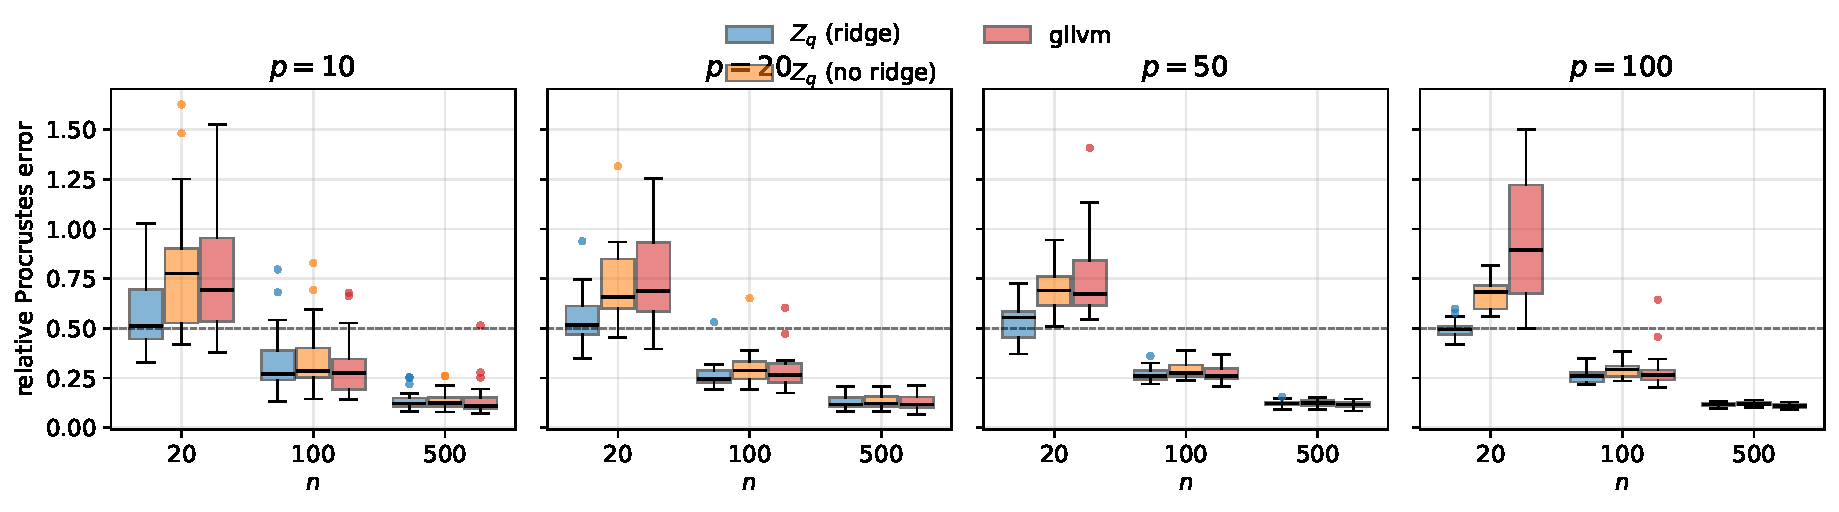
\includegraphics[width=\textwidth]{figures/sim1_procrustes_box.pdf}
\caption{Loading recovery in the MLE's own regime (dense Poisson, $q{=}2$, $\sigma_W{=}0.5$, $20$ replications; relative orthogonal Procrustes error, lower is better; fliers shown). $Z_q$ (with the asymptotically-free loading ridge) and \texttt{gllvm} are competitive in the median across the grid. When information is scarce ($n{=}20$) both are stressed; \texttt{gllvm} shows a heavy tail of catastrophic fits---fliers above the dashed line at $0.5$, i.e.\ loadings essentially orthogonal to the truth---most severely at small $n$ and large $p$, while the penalized $Z_q$ has a comparable or lighter spread.}
\label{fig:sim1box}
\end{figure}

\subsection{Robustness to outlier contamination}
\label{sec:exp-robust}
Because the statistic $T$ is ours to choose, bounded influence in the response is a one-line design choice---and the model-expectation centering $\mathbb E_\theta[T\cdot\eta]$ supplies the Fisher-consistency correction for \emph{any} $T$ automatically, so robustness costs no consistency. We fit a fixed clean Poisson GLLVM ($q{=}2,p{=}50,n{=}200$) and corrupt a fraction $\varepsilon$ of cells to a gross value $M$, fitting three estimators to the \emph{same} contaminated data that differ only in their influence: \texttt{gllvm} (full likelihood, unbounded influence in $y$); $Z_q$ with $T=\log(1+y)$ (logarithmic, down-weighted); and $Z_q$ with the bounded statistic $T=\min(\log(1+y),c)$, $c$ a robust cut estimated in log-space.

The bounded estimator is \emph{flat against outlier magnitude}: increasing $M$ from $10$ to $10^5$ leaves it at Procrustes $\approx 0.28$, while \texttt{gllvm} explodes (to $42$ and then numerical failure) and even the logarithmic $Z_q$ climbs (Table~\ref{tab:robust}, top). Against the contamination \emph{fraction} it is controlled up to a breakdown point near $\varepsilon\approx 0.3$---where the robust scale $c$ itself is corrupted (Table~\ref{tab:robust}, bottom). This is the constructive form of the robustness--efficiency trade-off: bounded influence by design, consistency by centering.

\begin{table}[t]
\centering
\caption{Robustness (clean Poisson $q{=}2,p{=}50,n{=}200$; Procrustes error). Top: outlier magnitude $M$ at fixed $\varepsilon{=}0.05$. Bottom: contamination fraction $\varepsilon$ at fixed $M{=}1000$. ``--'' = numerical failure.}
\label{tab:robust}
\begin{tabular}{lccccc}
\toprule
$M$ & $10$ & $100$ & $10^3$ & $10^4$ & $10^5$\\
\midrule
\texttt{gllvm}                 & $0.31$ & $1.38$ & $41.9$ & $24.3$ & --\\
$Z_q$ ($\log1p$)               & $0.22$ & $0.28$ & $0.42$ & $0.76$ & $1.40$\\
$Z_q$ (bounded $T$)            & $0.23$ & $0.28$ & $0.28$ & $0.28$ & $0.28$\\
\midrule
$\varepsilon$ & $0.02$ & $0.05$ & $0.10$ & $0.20$ & $0.30$\\
\midrule
\texttt{gllvm}                 & $8.3$  & $41.9$ & $30.6$ & $28.8$ & $69.0$\\
$Z_q$ ($\log1p$)               & $0.24$ & $0.42$ & $0.53$ & $0.69$ & $0.89$\\
$Z_q$ (bounded $T$)            & $0.19$ & $0.28$ & $0.39$ & $0.62$ & $1.11$\\
\bottomrule
\end{tabular}
\end{table}

\subsection{Scaling and a spatial-transcriptomics application}
\label{sec:exp-gp}
We now turn to the GP-GLLVM of Section~\ref{sec:gpgllvm}, the regime in which likelihood-based and variational methods do not apply.

\paragraph{Cost is independent of $n$.}
On synthetic data ($q{=}2$, $p{=}30$, squared-exponential kernel), fitting on random $K$-subsets ($K{=}15$) gives a wall-clock time that is \emph{flat} in the number of observations: groups of size up to $G{=}1000$ with $B{=}2000$ groups---up to several million observations---fit in about $3.5$ seconds, with recovery improving as $G$ grows. By contrast a full-group Gaussian-process likelihood is $O(G^3)$ and, with a non-Gaussian latent, intractable. The per-factor length-scales are recovered cleanly: with distinct true scales $\ell=(1,3)$, ten cold-start runs on fresh data give $\hat\ell=(1.01\pm0.03,\,3.02\pm0.08)$ and loading error $0.027$, with no divergence.

\paragraph{Real data: 10x Visium mouse brain.}
We fit the GP-GLLVM to a 10x Visium spatial-transcriptomics section of mouse brain: $n=2695$ spots, $p=100$ spatially variable genes, Poisson responses, and $d=2$ spatial coordinates, with a per-spot library-size offset. Fitting on local spatial $K$-subsets takes about two minutes on a CPU and recovers \emph{distinct per-factor spatial length-scales} ranging from $\sim\!150\,\mu$m to $\sim\!1.5\,$mm. The corresponding factor maps (Figure~\ref{fig:visium}) are spatially coherent and anatomically interpretable, and their smoothness tracks the estimated length-scale---a scale-resolved, count-native decomposition of the tissue. The factor whose length-scale falls below the spot pitch is, correctly, an unstructured (nugget) channel. To our knowledge no existing method delivers count-native Gaussian-process factor analysis at this scale: Gaussian-process factor analysis and its spatial descendants are Gaussian and $O(n^3)$-bound. The construction also composes with the regularizers of the base estimator (e.g.\ a group lasso on loading columns for automatic factor selection), which we do not pursue here.

\begin{figure}[t]
\centering
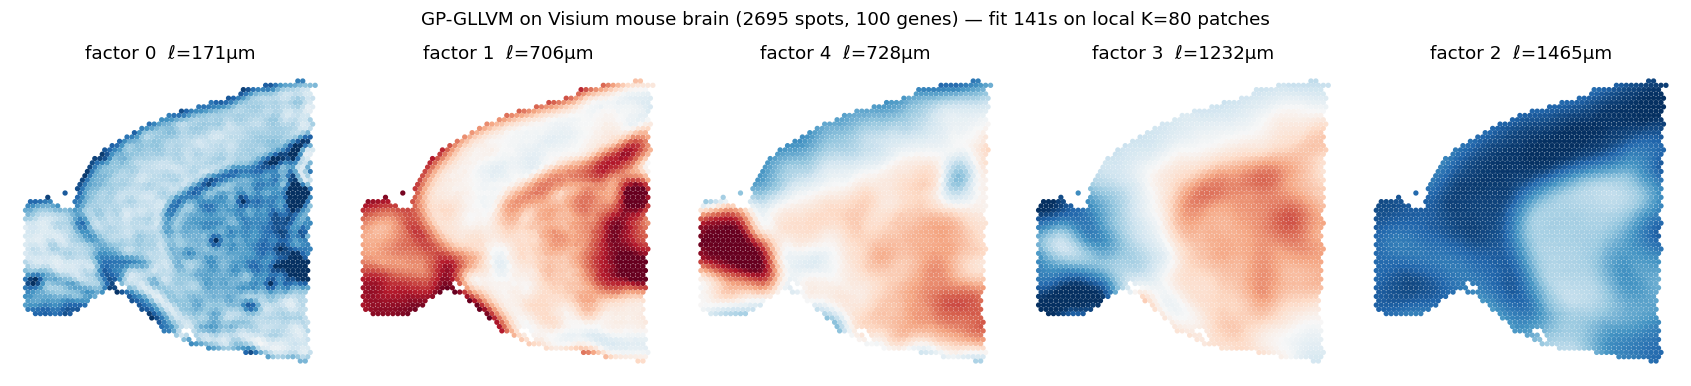
\includegraphics[width=\textwidth]{figures/visium_factors.png}
\caption{GP-GLLVM on 10x Visium mouse brain ($n{=}2695$ spots, $p{=}100$ genes), fit likelihood-free on local spatial $K$-subsets. Each panel is one estimated latent factor over the tissue, ordered by its recovered spatial length-scale $\ell$ (annotated). The factors form a scale-resolved decomposition---fine, near-resolution texture through broad anatomical gradients---with smoothness tracking $\ell$.}
\label{fig:visium}
\end{figure}

\paragraph{Summary.}
Across the four studies, $Z_q$ recovers the decoder where ELBO training is biased and is invariant to the response dimension (Section~\ref{sec:exp-misspec}); is competitive with the MLE in the MLE's own regime (Section~\ref{sec:exp-turf}); is robust to gross contamination by a one-line change of statistic (Section~\ref{sec:exp-robust}); and scales to a Gaussian-process latent model and real spatial data that lie beyond likelihood-based methods (Section~\ref{sec:exp-gp}).

\iffalse  % ===== superseded simulation/results section (kept for reference) =====
% ------------------------------------------------
% SIMULATION
%
\section{Simulation study}

\subsection{intro to sims}

First setting: robustness to crude but scalable surrogates.
This is the “I only have a cheap wrong inference mechanism, can I still estimate the decoder?” case. It shows your method is not tied to high-quality approximate posteriors. That is important because it demonstrates robustness to serious misspecification in a practically relevant large-scale regime.

Second setting: robustness to encoder reuse under shift.
This should probably be the flagship experiment. It is the cleanest embodiment of the paper’s main message. A surrogate learned on one population is reused on another; naive decoder learning breaks; centering repairs the target and remains stable over a meaningful drift range. This is likely the most memorable setting.

Third setting: correction under encoder underspecification.
This is the “ordinary VAE reality” experiment. Even without dramatic shift or bizarre imputers, the encoder family may just be too weak. Then your method becomes a correction/refinement step for decoder estimation. This broadens the paper beyond special regimes and makes it relevant to standard amortized inference practice.

\subsection{Main sims}
\label{sec:sims}


Our approach decouples decoder estimation from posterior accuracy by treating the surrogate posterior 
as a nuisance object within a centered Z-estimation framework. Rather than requiring the surrogate
to approximate the true posterior, we only require that the resulting estimating equations remain locally identifying. This allows decoder parameters to be estimated consistently using extremely crude inference schemes, including deterministic solvers such as MAP imputation or encoders trained under misspecified models.

We emphasize two practically relevant regimes. First, in parametric latent variable models where posterior inference is computationally prohibitive—such as high-dimensional or longitudinal GLLVMs—we show that decoder consistency can be recovered by plugging in a fixed, possibly wrong, latent estimator and centering the estimating equations appropriately. This enables scalable estimation in settings where likelihood-based or variational methods are infeasible.

Second, we consider transfer and distribution-shift scenarios in which an encoder is pretrained on a large reference dataset and subsequently frozen. While standard ELBO-based updates yield biased decoder estimates under such encoder reuse, the proposed $Z_q$ estimator remains consistent by construction, provided a mild Jacobian condition holds.

Finally, we include a small neural-network illustration on handwritten digits to demonstrate that the same principles apply in amortized inference settings, without making neural architectures the focus of the paper.


We evaluate the proposed $Z_q$ estimator in controlled settings where the data-generating process is fully known.  The simulation design targets the two central claims of the paper: (i) \emph{decoder consistency} under arbitrary surrogate posteriors $q_{\Z\mid\Y}$ (including severely misspecified, pretrained, or underspecified encoders), and (ii) a \emph{robustness--efficiency trade-off}, where poorer surrogates increase variance but do not induce asymptotic bias, provided the Jacobian condition holds.

Across all experiments, we generate i.i.d.\ samples $\{\Y_i\}_{i=1}^n$ from a latent-variable model with true decoder parameter $\bt_0$.  We then fit the model using two learning rules:
(i) a baseline variational approach that updates $\bt$ by maximizing an ELBO built from a surrogate posterior $q_{\Z\mid\Y}$ (amortized or otherwise), and
(ii) the proposed $Z_q$ procedure that updates $\bt$ by solving the centered estimating equations $\Psi_{n;q}(\bt)=0$ using the same surrogate $q_{\Z\mid\Y}$.

To isolate the effect of posterior misspecification, we separate \emph{inference} (how $q_{\Z\mid\Y}$ is obtained) from \emph{estimation} (how $\bt$ is updated).  In particular, several experiments deliberately fix or degrade $q_{\Z\mid\Y}$ while keeping the data-generating model correctly specified.

\paragraph{Common protocol.}
Each experiment follows the same steps:
\begin{enumerate}
\item \textbf{Data generation.} Choose $(f_\Z, f_{\Y\mid\Z;\bt_0})$ and simulate $\Z_i \sim f_\Z$ and $\Y_i\mid\Z_i \sim f_{\Y\mid\Z;\bt_0}$ for $i=1,\dots,n$.
\item \textbf{Surrogate posterior construction.} Construct a surrogate $q_{\Z\mid\Y}$ (amortized encoder, frozen encoder, point imputation, Laplace/MAP, or a deliberately wrong model), possibly trained on a different dataset or under a misspecified model.
\item \textbf{Decoder estimation.} Fit $\bt$ using (a) ELBO-based learning with $q_{\Z\mid\Y}$ and (b) $Z_q$ learning with the \emph{same} $q_{\Z\mid\Y}$.
\item \textbf{Repetition and metrics.} Repeat over $R$ Monte Carlo replications and report decoder error, bias/variance behavior, and (when relevant) coverage using the variance estimation procedure of Section~\ref{sec:variance}.
\end{enumerate}

\paragraph{Metrics.}
Let $\hat\bt$ denote an estimator of $\bt_0$.  We report (i) a parameter error such as $\|\hat\bt-\bt_0\|$ (or blockwise relative error for loading matrices), (ii) empirical bias and variance over replications, and (iii) when applicable, Wald-type coverage based on an estimated covariance matrix.


\subsection{Experiment A: wrong-model MAP imputation}
\label{sec:simA}

We first consider a setting where the surrogate posterior is obtained by point imputation under a \emph{misspecified} model.  This mimics practical workflows where latent variables are approximated by a fast imputer or by a legacy inference pipeline that does not match the current generative specification.

\paragraph{Steps.}
\begin{enumerate}
\item \textbf{Generate data.} Fix a GLLVM with latent dimension $q$ and mixed outcomes (Gaussian/Poisson/Bernoulli) and draw $\Z_i \sim f_\Z$, $\Y_i\mid \Z_i \sim f_{\Y\mid\Z;\bt_0}$.
\item \textbf{Build a wrong imputer.} Specify an \emph{incorrect} latent model $\tilde f_{\Y,\Z;\tilde\bt}$ (e.g., wrong link functions, wrong variance structure, wrong prior, or wrong $q$). Fit $\tilde\bt$ by a crude method (or fix it).
\item \textbf{Define $q_{\Z\mid\Y}$.} For each $\Y_i$, compute a MAP estimate $\tilde z_i = \arg\max_z \tilde f_{\Z\mid\Y;\tilde\bt}(z\mid \Y_i)$ and set $q_{\Z\mid\Y}(\cdot\mid \Y_i)=\delta_{\tilde z_i}(\cdot)$.
\item \textbf{Estimate $\bt$.} Using this degenerate surrogate $q_{\Z\mid\Y}$, fit $\bt$ by (a) ELBO/variational learning (using $\delta_{\tilde z_i}$) and (b) $Z_q$ estimation.
\item \textbf{Evaluate.} Compare $\hat\bt$ to $\bt_0$ over replications and sample sizes.
\end{enumerate}


\subsection{Experiment B: encoder underspecification sweep}
\label{sec:simB}

We next isolate the impact of amortized posterior quality by fitting a correctly specified GLLVM while systematically reducing encoder capacity.  This experiment targets amortization/underspecification bias: restricted encoder families yield biased decoder gradients under ELBO training, and this bias typically persists as $n$ grows.

\paragraph{Steps.}
\begin{enumerate}
\item \textbf{Generate data.} Simulate $\Z_i$ and $\Y_i$ from the same GLLVM as in Experiment~\ref{sec:simA}, with true parameter $\bt_0$.
\item \textbf{Train encoder family.} For a grid of capacities $h\in\mathcal H$ (e.g.\ hidden width or bottleneck size), train an amortized encoder $q_{\phi_h}(\Z\mid\Y)$ within a fixed variational family (e.g.\ diagonal Gaussian).
\item \textbf{Fit $\bt$ with shared $q$.} For each $h$, estimate $\bt$ by:
(a) standard VAE/ELBO optimization using $q_{\phi_h}$, and
(b) $Z_q$ updates using the same $q_{\phi_h}$.
\item \textbf{Evaluate bias/variance.} For each $h$, report parameter error and decompose the empirical behavior into bias (drift of the mean) and variance (spread across replications).
\end{enumerate}



\subsection{Experiment C: frozen encoder under decoder shift}
\label{sec:simC}

We then study encoder reuse under distribution shift.  An encoder is trained on a source model and then frozen.  On a target dataset generated from a different decoder parameter, we re-estimate only $\bt$.  This directly tests whether decoder learning remains valid when $q_{\Z\mid\Y}$ is mismatched to the target population.

\paragraph{Steps.}
\begin{enumerate}
\item \textbf{Source training.} Generate a source dataset from $(f_\Z, f_{\Y\mid\Z;\bt_{\mathrm{src}}})$ and train an amortized encoder $q_{\phi}(\Z\mid\Y)$ (e.g.\ by ELBO).
\item \textbf{Freeze $q$.} Fix $\phi$ and treat $q_{\Z\mid\Y}=q_{\phi}$ as a black box.
\item \textbf{Target generation.} Generate a target dataset from the same model class but with $\bt_0=\bt_{\mathrm{tgt}}\neq \bt_{\mathrm{src}}$.
\item \textbf{Re-estimate $\bt$.} On the target dataset, estimate $\bt$ using (a) ELBO learning with frozen $q_{\phi}$ and (b) $Z_q$ with the same frozen $q_{\phi}$.
\item \textbf{Evaluate.} Compare decoder recovery across the shift magnitude $\|\bt_{\mathrm{tgt}}-\bt_{\mathrm{src}}\|$ and sample size $n$.
\end{enumerate}

\subsection{Experiment D: MNIST encoder reuse (digits 0--8 $\to$ 9)}
\label{sec:simD}

Finally, we consider a high-dimensional benchmark where encoder reuse is natural.  We train an encoder on digits $0$--$8$ and freeze it.  We then fit a decoder on digit $9$ only, comparing standard VAE learning to $Z_q$.  This setting tests whether decoder learning remains well-behaved when inference is transferred from a related but non-identical population.

\paragraph{Steps.}
\begin{enumerate}
\item \textbf{Train on digits 0--8.} Fit a VAE on MNIST restricted to labels $\{0,\dots,8\}$, obtaining an encoder $q_{\phi}(\Z\mid\Y)$.
\item \textbf{Freeze encoder.} Keep $\phi$ fixed and discard (or reinitialize) the decoder.
\item \textbf{Fit on digit 9.} Using only digit $9$ images, estimate decoder parameters $\bt$ via (a) ELBO learning with frozen $q_{\phi}$ and (b) $Z_q$ updates with the same frozen $q_{\phi}$.
\item \textbf{Evaluate generative quality.} Compare samples from the fitted decoders and quantitative metrics (e.g.\ reconstruction on held-out 9s, likelihood proxies, or classifier-based scores).
\end{enumerate}






\section{Results}
\label{sec:results}

We evaluate the proposed $Z_q$ estimator from both a theoretical and empirical
perspective.  Our results highlight three main findings:  
(i) the centered estimating equations restore consistency under severe posterior
misspecification;  
(ii) this robustness comes with a controlled loss of efficiency that matches the
theoretical trade-off characterized in Section~\ref{sec:zq_estimator};  
(iii) in practical settings with amortized or reused encoders, $Z_q$ yields stable
decoder estimates in regimes where standard variational methods fail.


\subsection{Theoretical implications}

The asymptotic results of Section~\ref{sec:asymptotics} show that decoder
consistency does not require the surrogate posterior $q_{\Z\mid\Y}$ to be correct.
Rather, consistency follows from two ingredients: centering, which guarantees that
the population moment vanishes at $\bt_0$, and local nonsingularity of the induced
Jacobian. In particular, Theorem~\ref{thm:Zq-main} shows that any solution of the
centered estimating equations is consistent and asymptotically normal under the
stated regularity conditions.

A direct consequence is that posterior misspecification affects the
\emph{efficiency} of the estimator, not the location of the population root.
When the surrogate is close to the true posterior, the induced estimating equations
tend to be better conditioned and less variable. When the surrogate is poor, the
asymptotic variance may increase, as reflected in the sandwich covariance of
Theorem~\ref{thm:Zq-main}. What centering removes is asymptotic bias from the
population target, not necessarily all efficiency loss relative to maximum
likelihood.

The perturbation argument of Section~\ref{sec:asymptotics} further clarifies the
robustness regime. The Jacobian is a perturbation of the Fisher information, so
substantial approximation error is still admissible provided it does not destroy
local nonsingularity. This explains why $Z_q$ remains stable even with crude or
underspecified surrogates.

\subsection{Synthetic experiments: GLLVMs}

We first study generalized linear latent variable models (GLLVMs) for which the
true data-generating process is known.  Latent variables are Gaussian and
observations include mixed Poisson, Binomial, and Gaussian responses.  This setting
allows us to isolate the effect of posterior misspecification while keeping the
decoder correctly specified.

We consider a sequence of increasingly misspecified encoders, ranging from
high-capacity amortized networks to extreme point-imputation schemes.  For each
encoder, we compare standard variational inference (joint ELBO optimization) with
decoder updates based on the $Z_q$ estimating equations.

Across all settings, variational inference exhibits growing bias as encoder
capacity decreases: decoder parameter estimates drift away from the truth even as
the sample size increases.  In contrast, the $Z_q$ estimator remains centered around
$\bt_0$ for all encoder qualities.  While the variance of the estimates increases
with posterior misspecification, no systematic bias is observed.  These findings
are consistent with the theoretical predictions and illustrate the robustness of
the centered estimating equations.

\subsection{Amortized inference under encoder reuse}

We next consider a transfer-learning scenario in which an encoder trained on a
source dataset is reused without retraining on a target dataset.  Such settings
are common in applications where inference is expensive or data are scarce.

We train an encoder on simulated data generated from a reference model and then
freeze it.  On new datasets with different decoder parameters, we estimate the
decoder using either the frozen encoder with standard ELBO gradients or with the
$Z_q$ updates.  Despite the encoder being mismatched to the target distribution,
the $Z_q$ estimator consistently recovers the correct decoder parameters, whereas
ELBO-based updates exhibit persistent bias.

These results confirm that $Z_q$ decouples encoder quality from decoder
consistency, enabling safe reuse of pretrained or externally provided inference
modules.

\subsection{Efficiency--robustness trade-off}

Finally, we empirically examine the efficiency trade-off implied by the theory.
When the approximate posterior is accurate, the variance of the $Z_q$ estimator is
close to that of the maximum likelihood estimator.  As the posterior approximation
deteriorates, variance increases smoothly, reflecting the degradation of the
Jacobian condition.  Importantly, no abrupt instability is observed: even severely
misspecified posteriors yield well-behaved estimating equations.

Taken together, these results demonstrate that the proposed $Z_q$ estimator
achieves reliable decoder estimation across a wide range of inference regimes,
including settings in which standard variational approaches are known to fail.

\fi  % ===== end superseded simulation/results section =====



\section{Extension: low-dimensional inference with frozen nuisance components}

The present framework also suggests a natural extension to settings in which the decoder is partly high-dimensional but the parameter of substantive interest is low-dimensional. Suppose, for example, that the natural parameter takes the form
\[
\eta(x,z;\gamma,\beta)
=
g_\gamma(x,z)+\beta\,t,
\]
where \(g_\gamma\) is a flexible nuisance component, such as a neural network, and \(\beta\) is a scalar treatment effect. In such a setting, one may imagine training the encoder and the nuisance decoder component \(g_\gamma\), then freezing both and applying centered estimating equations only to \(\beta\).

This would be attractive in applications where the main goal is inference on a small interpretable parameter rather than estimation of the full decoder. The resulting procedure would retain the modularity emphasized in this paper: the encoder and the high-dimensional nuisance component would serve as frozen surrogate mechanisms, while inference would target only the low-dimensional parameter of interest.

A full treatment of this extension lies beyond the scope of the present work. In particular, once the nuisance components are themselves learned from data, valid inference for \(\beta\) would require additional arguments controlling the effect of nuisance estimation, potentially through orthogonality or sample-splitting ideas. Still, the centered construction developed here provides a natural starting point for such a theory.


% ----------------------------------

\newpage
\bibliography{references} 
\newpage
\appendix

\section{Mathematical Appendix}
\label{appendix:theory}

This appendix collects the main derivations used in the paper. We work throughout under the regularity conditions required to interchange differentiation and integration, and we assume all expectations below are well defined.

\subsection{From the marginal log-likelihood to the MLE estimating equations}
\label{apx:mle-estimating-equations}

Recall that the marginal density of \(\Y\) is
\[
f_{\Y;\bt}(\y)
=
\int_{\mathcal Z} f_{\Y,\Z;\bt}(\y,\z)\,d\z,
\]
where
\[
f_{\Y,\Z;\bt}(\y,\z)
=
f_{\Y\mid\Z;\bt}(\y\mid \z)\,f_\Z(\z).
\]
For a single observation \(\y\), the marginal log-likelihood is
\[
\ell(\bt;\y)
=
\log f_{\Y;\bt}(\y)
=
\log \int_{\mathcal Z} f_{\Y,\Z;\bt}(\y,\z)\,d\z.
\]
Differentiating with respect to \(\bt\) gives
\begin{align}
\nabla_\bt \ell(\bt;\y)
&=
\frac{\nabla_\bt f_{\Y;\bt}(\y)}{f_{\Y;\bt}(\y)}
\nonumber\\
&=
\frac{\int_{\mathcal Z} \nabla_\bt f_{\Y,\Z;\bt}(\y,\z)\,d\z}{f_{\Y;\bt}(\y)}.
\label{eq:appendix_score_step1}
\end{align}
Using
\[
\nabla_\bt f_{\Y,\Z;\bt}(\y,\z)
=
f_{\Y,\Z;\bt}(\y,\z)\,\nabla_\bt \log f_{\Y,\Z;\bt}(\y,\z),
\]
we obtain
\begin{align}
\nabla_\bt \ell(\bt;\y)
&=
\frac{\int_{\mathcal Z} f_{\Y,\Z;\bt}(\y,\z)\,\nabla_\bt \log f_{\Y,\Z;\bt}(\y,\z)\,d\z}{f_{\Y;\bt}(\y)}
\nonumber\\
&=
\int_{\mathcal Z}
\nabla_\bt \log f_{\Y,\Z;\bt}(\y,\z)\,
\frac{f_{\Y,\Z;\bt}(\y,\z)}{f_{\Y;\bt}(\y)}
\,d\z
\nonumber\\
&=
\mathbb E_{f_{\Z\mid\Y;\bt}(\cdot\mid \y)}
\!\left[
\nabla_\bt \log f_{\Y,\Z;\bt}(\y,\Z)
\right].
\label{eq:appendix_score_identity}
\end{align}
This proves the posterior representation of the marginal score:
\[
s(\bt;\y)
=
\nabla_\bt \log f_{\Y;\bt}(\y)
=
\mathbb E_{f_{\Z\mid\Y;\bt}(\cdot\mid \y)}
\!\left[
\nabla_\bt \log f_{\Y,\Z;\bt}(\y,\Z)
\right].
\]
For i.i.d.\ observations \(\y_1,\dots,\y_n\), the maximum likelihood estimator is therefore a root of
\[
\frac1n\sum_{i=1}^n s(\bt;\y_i)=0,
\]
which is equation~\eqref{eq:mle_score_eq} in the main text.

\subsection{Exponential-family score decomposition}
\label{apx:expfam-score-decomp}

Suppose
\[
f_{\Y\mid\Z;\bt}(\y\mid \z)
=
\exp\!\left\{
T(\y)^\top \eta(\z,\bt)
-
A\!\bigl(\eta(\z,\bt)\bigr)
+
B(\y)
\right\}.
\]
Since \(f_\Z\) does not depend on \(\bt\), the complete-data log-density is, up to the prior term,
\[
\log f_{\Y,\Z;\bt}(\y,\z)
=
T(\y)^\top \eta(\z,\bt)
-
A\!\bigl(\eta(\z,\bt)\bigr)
+
B(\y)
+
\log f_\Z(\z).
\]
Differentiating with respect to \(\bt\) yields
\begin{align}
\nabla_\bt \log f_{\Y,\Z;\bt}(\y,\z)
&=
\frac{\partial \eta(\z,\bt)}{\partial \bt}^\top T(\y)
-
\frac{\partial \eta(\z,\bt)}{\partial \bt}^\top \nabla_\eta A\!\bigl(\eta(\z,\bt)\bigr)
\nonumber\\
&=
D(\z;\bt)^\top\bigl(T(\y)-\mu(\z;\bt)\bigr),
\label{eq:appendix_complete_score_expfam}
\end{align}
where
\[
D(\z;\bt)
=
\frac{\partial \eta(\z,\bt)}{\partial \bt},
\qquad
\mu(\z;\bt)
=
\nabla_\eta A\!\bigl(\eta(\z,\bt)\bigr)
=
\mathbb E_{f_{\Y\mid\Z;\bt}(\cdot\mid \z)}[T(\Y)].
\]
Substituting \eqref{eq:appendix_complete_score_expfam} into the posterior score identity \eqref{eq:appendix_score_identity} gives
\[
s(\bt;\y)
=
\mathbb E_{f_{\Z\mid\Y;\bt}(\cdot\mid \y)}
\!\left[
D(\Z;\bt)^\top\bigl(T(\y)-\mu(\Z;\bt)\bigr)
\right],
\]
which is equation~\eqref{eq:score_expfam} in the main text. Expanding the difference gives
\[
s(\bt;\y)
=
\mathbb E_{f_{\Z\mid\Y;\bt}(\cdot\mid \y)}
\!\bigl[D(\Z;\bt)^\top T(\y)\bigr]
-
\mathbb E_{f_{\Z\mid\Y;\bt}(\cdot\mid \y)}
\!\bigl[D(\Z;\bt)^\top \mu(\Z;\bt)\bigr],
\]
which is equation~\eqref{eq:score_two_terms}.

\subsection{Differentiation identity for model-based expectations}
\label{apx:diff-identity}

Let \(g(\bt,\Y)\) be any measurable function for which differentiation under the integral sign is justified. Then
\[
\mathbb E_{f_{\Y;\bt}}\!\left[g(\bt,\Y)\right]
=
\int g(\bt,\y)\,f_{\Y;\bt}(\y)\,d\y.
\]
Differentiating with respect to \(\bt\) gives
\begin{align}
\nabla_\bt \mathbb E_{f_{\Y;\bt}}\!\left[g(\bt,\Y)\right]
&=
\int \nabla_\bt g(\bt,\y)\,f_{\Y;\bt}(\y)\,d\y
+
\int g(\bt,\y)\,\nabla_\bt f_{\Y;\bt}(\y)\,d\y
\nonumber\\
&=
\mathbb E_{f_{\Y;\bt}}\!\left[\nabla_\bt g(\bt,\Y)\right]
+
\mathbb E_{f_{\Y;\bt}}\!\left[
g(\bt,\Y)\,
\frac{\nabla_\bt f_{\Y;\bt}(\Y)}{f_{\Y;\bt}(\Y)}
\right]
\nonumber\\
&=
\mathbb E_{f_{\Y;\bt}}\!\left[\nabla_\bt g(\bt,\Y)\right]
+
\mathbb E_{f_{\Y;\bt}}\!\left[g(\bt,\Y)s(\bt;\Y)^\top\right],
\label{eq:appendix_diff_identity}
\end{align}
where \(s(\bt;\Y)=\nabla_\bt \log f_{\Y;\bt}(\Y)\) is the marginal score.

\subsection{Derivation of the Jacobian identity}
\label{apx:jacobian}

Recall that
\[
\psi(\bt;\y)
=
\mathbb E_{q_{\Z\mid\Y;\bt}(\cdot\mid \y)}
\!\left[
D(\Z;\bt)^\top T(\y)
\right]
\]
and
\[
\Psi(\bt)
=
\mathbb E_{f_{\Y;\bt_0}}\!\left[\psi(\bt;\Y)\right]
-
\mathbb E_{f_{\Y;\bt}}\!\left[\psi(\bt;\Y)\right].
\]
Differentiating \(\Psi(\bt)\) gives
\begin{align}
\nabla_\bt \Psi(\bt)
&=
\mathbb E_{f_{\Y;\bt_0}}\!\left[\nabla_\bt \psi(\bt;\Y)\right]
-
\nabla_\bt \mathbb E_{f_{\Y;\bt}}\!\left[\psi(\bt;\Y)\right].
\label{eq:appendix_jacobian_step1}
\end{align}
Applying the identity \eqref{eq:appendix_diff_identity} with \(g(\bt,\Y)=\psi(\bt;\Y)\) yields
\begin{align}
\nabla_\bt \mathbb E_{f_{\Y;\bt}}\!\left[\psi(\bt;\Y)\right]
&=
\mathbb E_{f_{\Y;\bt}}\!\left[\nabla_\bt \psi(\bt;\Y)\right]
+
\mathbb E_{f_{\Y;\bt}}\!\left[\psi(\bt;\Y)s(\bt;\Y)^\top\right].
\label{eq:appendix_jacobian_step2}
\end{align}
Substituting \eqref{eq:appendix_jacobian_step2} into \eqref{eq:appendix_jacobian_step1}, we obtain
\begin{align}
\nabla_\bt \Psi(\bt)
&=
\mathbb E_{f_{\Y;\bt_0}}\!\left[\nabla_\bt \psi(\bt;\Y)\right]
-
\mathbb E_{f_{\Y;\bt}}\!\left[\nabla_\bt \psi(\bt;\Y)\right]
-
\mathbb E_{f_{\Y;\bt}}\!\left[\psi(\bt;\Y)s(\bt;\Y)^\top\right].
\end{align}
Evaluating at \(\bt=\bt_0\), the first two terms cancel:
\[
\nabla_\bt \Psi(\bt_0)
=
-
\mathbb E_{f_{\Y;\bt_0}}\!\left[\psi(\bt_0;\Y)s(\bt_0;\Y)^\top\right].
\]
Therefore
\[
A(\bt_0)
:=
-\nabla_\bt \Psi(\bt_0)
=
\mathbb E_{f_{\Y;\bt_0}}\!\left[\psi(\bt_0;\Y)s(\bt_0;\Y)^\top\right],
\]
which is equation~\eqref{eq:jacobian_final} in the main text.

\subsection{Full efficiency in Gaussian factor analysis}
\label{apx:fa-efficiency}

\begin{proposition}[Full efficiency in Gaussian factor analysis]
\label{prop:fa-efficiency}
Consider Gaussian factor analysis with
\[
\Y = \Lambda \Z + \varepsilon,
\qquad
\Z \sim \mathcal N(0,I_q),
\qquad
\varepsilon \sim \mathcal N(0,\Psi),
\]
where \(\Psi\) is diagonal and \(\theta=(\Lambda,\Psi)\). Let the surrogate posterior be the degenerate distribution
\[
q_{\Z\mid\Y}(\cdot\mid y)=\delta_{z_{\mathrm{MAP}}(y)}(\cdot),
\]
where \(z_{\mathrm{MAP}}(y)\) is the posterior mode of \(\Z\mid \Y=y\). Then the corresponding \(Z_q\) estimating equations coincide with the marginal score equations. Consequently, the \(Z_q\) estimator coincides with the maximum likelihood estimator and is Fisher efficient.
\end{proposition}

\begin{proof}
In Gaussian factor analysis, the conditional distribution of \(\Z\mid \Y=y\) is Gaussian with mean
\[
m_\theta(y)
=
\E_\theta[\Z\mid \Y=y]
=
(\Lambda^\top\Psi^{-1}\Lambda+I_q)^{-1}\Lambda^\top\Psi^{-1}y.
\]
Since the posterior is Gaussian, its mode equals its mean, so
\[
z_{\mathrm{MAP}}(y)=m_\theta(y).
\]

Write the complete-data log-likelihood, up to additive constants, as
\[
\ell_c(\theta;y,z)
=
-\frac12 (y-\Lambda z)^\top \Psi^{-1}(y-\Lambda z)
-\frac12 \log |\Psi|
-\frac12 z^\top z.
\]
Its score with respect to \(\theta\) is affine in \(z\) and \(zz^\top\). More explicitly, the score for \(\Lambda\) is
\[
S_\Lambda(\theta;y,z)
=
\Psi^{-1}(y-\Lambda z)z^\top,
\]
and the score for \(\Psi\) is
\[
S_\Psi(\theta;y,z)
=
-\frac12 \Psi^{-1}
+\frac12 \Psi^{-1}(y-\Lambda z)(y-\Lambda z)^\top \Psi^{-1},
\]
restricted to the diagonal coordinates of \(\Psi\).

The marginal score is obtained by taking conditional expectations under the true posterior:
\[
s(\theta;y)
=
\E_\theta\!\left[S(\theta;y,\Z)\mid \Y=y\right].
\]
Because \(\Z\mid \Y=y\) is Gaussian, we have
\[
\E_\theta[\Z\mid \Y=y]=m_\theta(y),
\qquad
\E_\theta[\Z\Z^\top\mid \Y=y]
=
\Var_\theta(\Z\mid \Y=y)+m_\theta(y)m_\theta(y)^\top.
\]
A direct calculation shows that, after centering by the model expectation as in the definition of \(Z_q\), the resulting estimating equations depend on the posterior only through these conditional moments. In the Gaussian factor-analysis model, these are exactly the moments generated by evaluating the affine score representation at the posterior mean \(m_\theta(y)\), together with the corresponding model-based centering term. Therefore taking the degenerate surrogate
\[
q_{\Z\mid\Y}(\cdot\mid y)=\delta_{m_\theta(y)}(\cdot)
\]
produces the same centered estimating equations as those induced by the exact posterior.

Hence the \(Z_q\) estimating equations coincide with the marginal score equations, so any root of the \(Z_q\) equations is an MLE. The estimator therefore coincides with the maximum likelihood estimator and inherits its Fisher efficiency.
\end{proof}


\subsection{Identification for the Gaussian-proxy GLLVM}
\label{apx:gllvm-identification}

We verify the local identification condition of Section~\ref{sec:asymptotics} for a concrete, widely used model. Consider a GLLVM with conditionally independent responses, each from a one-parameter exponential family with natural parameter $\eta_j(z;\bt)=w_j^\top z+b_j$, prior $\Z\sim\mathcal N(0,I_q)$, and $\bt=(W,b)$, $W=[w_1\mid\cdots\mid w_p]^\top$. The \emph{Gaussian proxy} takes a strictly increasing transform $T_j$ and treats $T_j(Y_j)\mid Z\sim\mathcal N(w_j^\top Z+b_j,\sigma^2)$, giving the closed-form MAP imputer
\[
\hat z(y;\bt)=\Sigma_z\,W^\top\!\big(T(y)-b\big),\qquad \Sigma_z=(W^\top W+\sigma^2 I)^{-1}.
\]
Write $\tilde T_j$ and $\tilde\mu_j(z)=\mathbb E[\tilde T_j(Y_j)\mid Z=z]$ for the family's canonical statistic and mean. By the Jacobian identity~\eqref{eq:jacobian_final}, $A(\bt_0)=\mathbb E[\psi(\bt_0;Y)\,s(\bt_0;Y)^\top]$, and the true marginal score decomposes response-by-response.

\begin{lemma}[Intercept block]
\label{lem:bblock}
For all $j\neq k$, $(A_{bb})_{jk}=0$, and for each $j$
\[
(A_{bb})_{jj}=\mathbb E\big[\operatorname{Cov}\!\big(T_j(Y_j),\,\tilde T_j(Y_j)\mid Z\big)\big]>0 .
\]
Thus $A_{bb}\succ0$, with no condition on $p$ or $W$.
\end{lemma}
\begin{proof}
$(A_{bb})_{jk}=\operatorname{Cov}\!\big(T_j(Y_j),\,s_{b_k}(\bt_0;Y)\big)$. Split the score residual $s_{b_k}=\big(\tilde T_k(Y_k)-\tilde\mu_k(Z)\big)+\big(\tilde\mu_k(Z)-\mathbb E[\tilde\mu_k(Z)\mid Y]\big)$. The first (noise) term has zero conditional mean given $Z$, so by the law of total covariance its covariance with $T_j(Y_j)$ equals $\mathbb E[\operatorname{Cov}(T_j(Y_j),\tilde T_k(Y_k)\mid Z)]$, which vanishes for $j\neq k$ by conditional independence and is the stated positive quantity for $j=k$ (strictly increasing $T_j$ and non-degenerate conditional variance). The second (posterior-residual) term is orthogonal in $L^2$ to every $\sigma(Y)$-measurable function, hence to $T_j(Y_j)$.
\end{proof}

\begin{lemma}[Loading block, large $p$]
\label{lem:wblock}
Let $p\to\infty$ with $q$ fixed and assume: \emph{(A1)} $\lambda_{\min}(W_p^\top W_p/p)\ge c>0$; \emph{(A2)} $\max_j\|w_j\|^2/p\to0$; \emph{(A3)} $\sup_j\operatorname{Var}(T_j(Y_j)\mid Z)\le\kappa<\infty$; \emph{(A4)} $\sup_j|\tilde\mu_j(Z)-(w_j^\top Z+b_j)|\le C\|w_j\|$. Then the MAP imputer concentrates, $\hat z(Y;\bt_0)=Z+O_{L^2}(p^{-1/2})$, and consequently the normalized Jacobian satisfies $A(\bt_0)/p=\mathcal I(\bt_0)/p+\bar R_p$ with $\|\bar R_p\|_{\mathrm{op}}=O(p^{-1/2})$; hence $A(\bt_0)$ is nonsingular for all $p$ large enough.
\end{lemma}
\begin{proof}[Proof sketch]
Decompose $T(Y)-b=WZ+\beta(Z)+\xi$ into signal, linearization bias $\beta_j=\tilde\mu_j(Z)-b_j-w_j^\top Z$, and conditional-mean-zero noise $\xi$. Then $\hat z-Z=-\sigma^2\Sigma_z Z+\Sigma_z W^\top\beta+\Sigma_z W^\top\xi$. Under (A1), $\|\Sigma_z\|_{\mathrm{op}}\le 1/(cp)$, giving shrinkage term $O(p^{-2})$ and, with (A4) and $\|W\|_F^2=O(p)$, bias term $O(p^{-1})$; the noise term has $\mathbb E\|\Sigma_z W^\top\xi\|^2\le\kappa\operatorname{tr}(\Sigma_z W^\top W\Sigma_z)\le\kappa q/(cp)$ by (A3). Hence $\mathbb E\|\hat z-Z\|^2=O(p^{-1})$. Both $\psi$ and $s$ are affine in $\hat z$ resp.\ $Z$ through the exponential-family structure, so $\psi-s=O_{L^2}(p^{-1/2})$ and, working with the per-feature objects $p^{-1/2}\psi,\;p^{-1/2}s$ (which have $O(1)$ norm), $\|\bar R_p\|_{\mathrm{op}}=O(p^{-1/2})$. Since $\lambda_{\min}(\mathcal I(\bt_0)/p)\ge c'>0$ under (A1), $A(\bt_0)/p=\mathcal I/p+\bar R_p$ is nonsingular once $p$ is large.
\end{proof}

\begin{proposition}[Local identification of the Gaussian-proxy GLLVM]
\label{prop:gllvm-id}
Let the $T_j$ be strictly increasing. Then: \textup{(i)} $A_{bb}(\bt_0)\succ0$ for all $p$ (Lemma~\ref{lem:bblock}); \textup{(ii)} $A(\bt_0)$ is nonsingular for all $p$ sufficiently large whenever $W$ has full column rank (Lemma~\ref{lem:wblock}); and \textup{(iii)} $A(\bt_0)$ is nonsingular whenever $\lambda_{\min}(\mathcal I(\bt_0))>\|A(\bt_0)-\mathcal I(\bt_0)\|_{\mathrm{op}}$, a condition verifiable numerically at any $\bt_0$. Under any of these, Theorem~\ref{thm:Zq-main} applies and the Gaussian-proxy $Z_q$ estimator is consistent and asymptotically normal with sandwich covariance $\Sigma=A^{-1}BA^{-\top}$.
\end{proposition}

\subsection{Identification of the GP-GLLVM}
\label{apx:gp-identification}

In the GP-GLLVM of Section~\ref{sec:gpgllvm} the latent covariance over a group is block-diagonal across factors, $\Sigma(\ell)=\operatorname{blkdiag}(K_{\ell_1},\dots,K_{\ell_q})$, with $K_{\ell_k}(t,t)=1$. Two distinct objects must not be conflated. \emph{(a) The instantaneous, within-observation cross-latent covariance} is the usual factor-analytic rotation gauge: it is absorbed into the loadings and is fixed by convention ($\operatorname{Cov}(Z_i)=I$). \emph{(b) The across-observation correlation}, i.e.\ the length-scales $\ell$, is a genuine estimand: the loadings act on a single $Z_i$ and are shared across observations, so they cannot encode how observations correlate over the coordinate.

The rotation gauge of the loadings depends on the kernels. Under a \emph{shared} kernel ($\ell_1=\cdots=\ell_q$), $\operatorname{Cov}(\operatorname{vec}Z)=K\otimes I_q$ is invariant under right-multiplication of $W$ by any $R\in O(q)$, so $W$ is identified only up to rotation and a triangular constraint is appropriate. Under \emph{distinct} length-scales, a rotation $R$ sends $\Sigma(\ell)$ to a covariance that is no longer block-diagonal in the same per-factor kernels unless $R$ merely permutes (and signs) factors with equal $\ell_k$; the gauge is therefore broken and $W$ is identified up to permutation and sign. Consequently a triangular constraint is, generically, \emph{misspecified} here: there is no rotation taking a full $W_0$ into triangular form while preserving the distinct-kernel covariance, so the constrained family excludes the truth and biases both $W$ and $\ell$. We therefore keep $W$ full. Factors whose length-scales coincide retain a residual rotation gauge among themselves (reflected as estimation variance in that subspace, not bias); the relative orthogonal Procrustes error, being rotation-invariant, is unaffected.


\subsection{Ridge stabilization and automatic penalty specification}
\label{apx:auto-lambda}

A loading-ridge penalty composes with the estimating equations at no cost to consistency. We add to the (sample-averaged) $Z_q$ objective a term $(\lambda/n)\|W\|_F^2$, so the estimating function in the loadings becomes
\[
\Psi_n^{\lambda}(\bt) \;=\; \Psi_n(\bt) \;-\; \frac{2\lambda}{n}\,\operatorname{vec}(W),
\]
where $\Psi_n$ is the unpenalized $Z_q$ function and $n$ the number of observations. Because $\Psi_n(\bt)$ is an $O_p(1)$ average while the penalty contributes a gradient of order $\lambda/n$, the perturbation vanishes as $n\to\infty$: the penalized root solves $\Psi_n(\bt)=2\lambda\,\operatorname{vec}(W)/n + o_p(n^{-1/2})$, and a first-order expansion around the unpenalized root $\widehat\bt$ gives $\widehat\bt^{\lambda}-\widehat\bt = O_p(\lambda/n)$. Since consistency and asymptotic normality are asymptotic statements, the $1/n$ scaling makes the penalized estimator share the same probability limit and the same first-order limiting distribution as the unpenalized one (Section~\ref{sec:asymptotics}); the ridge is therefore \emph{free} asymptotically. At finite $n$ it is not free, and that is its purpose: it bounds the loadings away from the runaway directions that destabilize the fit in the small-$n$, large-$q$, or overcomplete regimes, where the unregularized $Z_q$ surface is shallow. The penalty thus trades a finite-sample $O(\lambda/n)$ bias for a substantial variance reduction exactly where it is needed, and recedes where it is not. Figure~\ref{fig:ridge-bias} makes this concrete on the loading-recovery sweep of Section~\ref{sec:exp-turf}: pooling every loading element and regressing the residual on the true value, the ridge induces a mild shrinkage toward zero whose slope is $-0.15$ at $n{=}20$, $-0.04$ at $n{=}100$, and $-0.002$ at $n{=}500$---vanishing as $\lambda/n$ predicts---while the unpenalized \texttt{gllvm} is essentially unbiased throughout.

\begin{figure}[t]
\centering
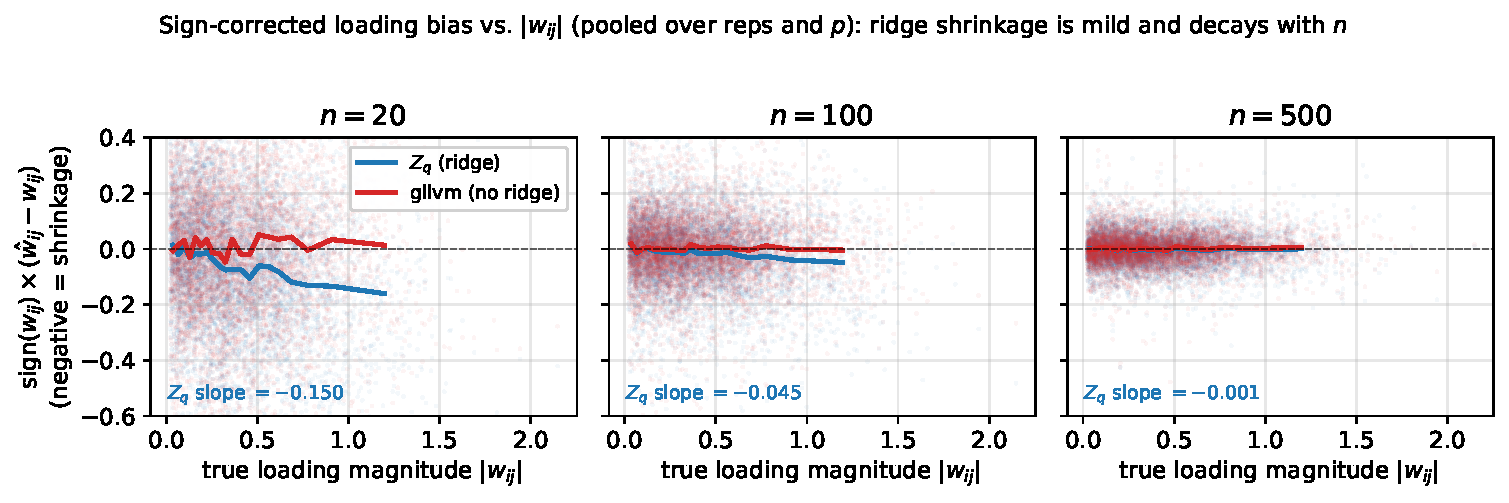
\includegraphics[width=\textwidth]{figures/sim1_bias.pdf}
\caption{Ridge-induced loading bias on the dense-Poisson sweep ($q{=}2$, $\sigma_W{=}0.5$): residual (estimate $-$ true) against the true loading value, pooled over replicates and response dimension $p$, with the equal-count binned mean overlaid. The $Z_q$ ridge ($\lambda{=}0.5$, penalty $0.5\,\|W\|_F^2/n$) shrinks loadings toward zero by an amount that decays with $n$ (slopes annotated), confirming the $O(\lambda/n)$ bias; \texttt{gllvm} (no ridge) is unbiased. The $y$-axis is clipped to expose the trend---the tail blow-ups of \texttt{gllvm} at small $n$ are shown in Figure~\ref{fig:sim1box}.}
\label{fig:ridge-bias}
\end{figure}

The constant $\lambda$ can be fixed once or chosen automatically, and the centered construction makes automatic selection essentially free. The fitted decoder is a fully specified generative model: at any current estimate $\widehat\bt$ we can simulate complete datasets $Y^\star \sim p_{\widehat\bt}$, for which the true loadings are \emph{known} (they are $\widehat W$ up to the gauge). Selecting $\lambda$ then requires no held-out data and no information criterion---it is a parametric bootstrap over the penalty:
\begin{enumerate}
\item simulate $B$ replicate datasets $Y^{\star (1)},\dots,Y^{\star (B)}$ of the observed size from $p_{\widehat\bt}$;
\item over a grid of candidate $\lambda$, refit each replicate and record the relative orthogonal Procrustes error to the known $\widehat W$;
\item set $\lambda^\star$ to the minimizer of the averaged error.
\end{enumerate}
This reuses exactly the model-expectation machinery already required by the centering term---the same ancestral draws and the same fit routine---so it adds only the cost of a small grid of refits, and it can be run on the fly once the estimate has settled. In the loading-recovery studies we instead fix a single value, $\lambda = 0.5$ (i.e.\ a penalty $0.5\,\|W\|_F^2/n$), stated once and used unchanged (the robustness experiment of Section~\ref{sec:exp-robust} uses no ridge); the automatic procedure above is the principled alternative when a default is undesirable, and the appendix sensitivity analysis confirms that the recovery is flat over a wide band of $\lambda$ and that $\lambda\to 0$ returns the unregularized fit.


\end{document}
